\documentclass[twocolumn]{article}

\usepackage[utf8]{inputenc}
\usepackage[T1]{fontenc}
\usepackage[english]{babel}
\usepackage{graphicx}
\usepackage{amsmath,amsfonts,amssymb}
\usepackage{hyperref}
\hypersetup{pdftitle={Classical and Deep Learning Approaches for White Blood Cell Classification}, pdfauthor={Th\'eophile Nadiedjoa}}
\usepackage{float}
\usepackage{times}
\usepackage{xcolor}
\usepackage{booktabs}
\usepackage{caption}
\usepackage{subcaption}
\usepackage{tikz}
\usepackage{array}
\usepackage{geometry}
\usepackage{listings}
\usepackage{enumitem}
\geometry{margin=2cm}
\graphicspath{{figures/}}

\usetikzlibrary{shapes.geometric, arrows.meta, positioning, fit, calc}

\usepackage[numbers,sort&compress]{natbib}

\lstset{
  basicstyle=\ttfamily\scriptsize,
  breaklines=true,
  frame=single,
  backgroundcolor=\color{gray!8}
}

\title{Classical and Deep Learning Approaches\\for White Blood Cell Classification\\from Peripheral Blood Smear Microscopy\\[0.5em]\large IMA205 Challenge --- Full Technical Report}
\author{Th\'eophile Nadiedjoa\\ T\'el\'ecom Paris}
\date{April 2026}

\begin{document}
\maketitle
\tableofcontents
\newpage

% ============================================================
\section*{Abstract}
\addcontentsline{toc}{section}{Abstract}
% ============================================================

White blood cell (WBC) classification from peripheral blood smear microscopy is a fundamental task in clinical hematology, yet remains challenging due to extreme class imbalance (ratio 1183:1 in our dataset), staining variability, and morphological similarity between cell subtypes. In this work, we systematically explore and compare two complementary paradigms on the IMA205 challenge (28,901 training images, 9,634 test images, 13 cell types).

\textbf{Part~I} presents a classical machine learning pipeline following the textbook recipe recommended by Al-Dulaimi et al.~\cite{aldulaimi2018}: Reinhard color normalization in LAB space, marker-controlled Watershed cell segmentation, Morphological Geodesic Active Contours (GAC) for nucleus refinement, then a $\sim$210-dimensional handcrafted feature vector (shape, color, texture via GLCM/LBP/HOG, Fourier descriptors), classified using SMOTE-balanced LightGBM, Random Forest, ExtraTrees, SVM-RBF, and Voting/Stacking ensembles under 5-fold stratified cross-validation, reaching macro-F1~=~0.509 (LightGBM, best of the six).

\textbf{Part~II} traces nine successive deep-learning iterations (\texttt{deep\_1}--\texttt{deep\_9}), each motivated by specific failures of the previous one. Starting from a vanilla EfficientNet-B3 baseline (single 85/15 validation split, macro-F1~=~0.552), we explored CBAM attention, late fusion with handcrafted morphometry, Wiener/Laplacian preprocessing, paper-based segmentation pipelines, before pivoting to ConvNeXt-Base with Focal Loss, CutMix/Mixup, and 2-phase fine-tuning. We document a critical data leakage pitfall (\texttt{deep\_5}: apparent F1=0.82, corrected to F1=0.70 in \texttt{deep\_6}), and present post-hoc experiments with ResNet50 (\texttt{deep\_7}), ResNeXt101 with multi-task learning (\texttt{deep\_8}), and a controlled ablation of handcrafted features (\texttt{deep\_9}). The deployed model is \texttt{deep\_9 no-morph} (no handcrafted features): \texttt{deep\_6}'s architecture plus a lightweight SE-style attention gate and HSV-V CLAHE preprocessing, achieving macro-F1 = 0.7052 / accuracy = 0.937 on validation -- the highest score of the 9 iterations, although within the noise of the validation split compared with \texttt{deep\_6} (0.6994).

Beyond raw scores, our results suggest that (1)~learned representations clearly outperform handcrafted features (0.699 for \texttt{deep\_6} on a held-out split vs.\ 0.509 in cross-validation for the classical pipeline), (2)~within the designs we tried, the ConvNeXt backbone mattered more than added modules: a similarly sized ResNeXt101 with CBAM and multi-task heads (\texttt{deep\_8}, 0.665) did not reach the plain ConvNeXt + MLP (0.699), and attention/fusion gave at most marginal gains, and (3)~a correct evaluation protocol is essential: splitting after oversampling inflated the validation score from 0.70 to 0.82.

% ============================================================
\section{Introduction}
% ============================================================

The differential white blood cell count is one of the most commonly ordered laboratory tests in clinical practice. It provides critical diagnostic information for conditions ranging from infections and allergies to leukemia and other hematological malignancies~\cite{aldulaimi2018}. Traditionally performed manually by trained hematologists examining Giemsa- or Wright-stained blood smears under a microscope, this process is time-consuming, subjective, and prone to inter-observer variability.

Automated WBC classification using computer vision has been an active area of research, with approaches spanning from classical image processing and handcrafted feature extraction~\cite{rezatofighi2011, gautam2014} to modern deep learning methods~\cite{tran2018, qin2018}. As highlighted by Al-Dulaimi et al.~\cite{aldulaimi2018} in their comprehensive survey, several critical challenges persist:

\begin{itemize}
    \item \textbf{Staining variability}: Different protocols (Giemsa, Wright, May-Gr\"unwald) lead to significant color variations.
    \item \textbf{Illumination differences}: Microscope lighting conditions vary between acquisitions.
    \item \textbf{Arbitrary cell orientation}: WBCs appear at any rotation angle on the slide.
    \item \textbf{Scale and position variations}: The nucleus and cytoplasm occupy varying proportions of the field of view.
    \item \textbf{Morphological similarity}: Several subtypes, particularly within the granulocyte lineage, share similar nuclear shapes.
\end{itemize}

In this work, we address these challenges through two complementary strategies. We first implement a classical ML pipeline to understand the discriminative value of explicit morphological features, then develop a deep learning pipeline through extensive iterative experimentation (9 iterations). This dual approach allows us to compare the strengths and limitations of each paradigm and document the lessons learned along the way.

% ============================================================
\section{Related Work}
\label{sec:relatedwork}
% ============================================================

The literature on WBC classification can be broadly organized into two families: \textbf{classical image analysis pipelines} and \textbf{representation-learning approaches}.

\paragraph{Classical pipelines.}
Early and still influential work relies on explicit segmentation and handcrafted descriptors. Typical pipelines isolate the nucleus and cytoplasm using thresholding, region growing, Watershed, K-Means, Active Contours, or morphological filtering, then extract shape/color/texture features (e.g., Hu moments, GLCM, LBP, Fourier descriptors) for conventional classifiers~\cite{rezatofighi2011, gautam2014, ghosh2010}. Rustam et al.~\cite{rustam2022} combine texture and RGB features with oversampling of the minority classes. The review by Al-Dulaimi et al.~\cite{aldulaimi2018} emphasizes that these approaches are interpretable and medically grounded, but strongly depend on segmentation quality and often degrade under staining/illumination variability.

\paragraph{Deep learning and attention mechanisms.}
More recent studies replace handcrafted features with end-to-end CNN feature learning~\cite{qin2018, tran2018}, usually via transfer learning to handle limited medical data; To\u{g}a\c{c}ar et al.~\cite{togacar2020} instead extract deep features from pretrained CNNs and feed a selected subset to conventional classifiers, a hybrid we also evaluate (CNN+SVM/RF). Attention modules (e.g., CBAM, SE) have been proposed to improve focus on discriminative regions~\cite{woo2018cbam, hu2018squeeze}. In practice, gains are task-dependent and often smaller than expected when the baseline backbone is already strong.

\paragraph{Positioning of this work.}
Our report follows this evolution explicitly: Part~I implements a robust classical pipeline inspired by the survey recommendations~\cite{aldulaimi2018}, while Part~II evaluates modern transfer-learning pipelines (EfficientNet/ConvNeXt/ResNet/ResNeXt), attention variants, and hybrid fusion with handcrafted features. This design enables a controlled comparison between interpretability-oriented classical vision and high-capacity learned representations.

% ============================================================
\section{Dataset}
% ============================================================

\subsection{Overview}

The challenge dataset consists of 28,901 training images and 9,634 test images of individual white blood cells captured from peripheral blood smear microscopy. Images are $368\times368$ or $368\times370$ RGB images (JPEG-encoded, with a \texttt{.png} extension). The challenge is modelled on the public WBCBench 2026 benchmark~\cite{wbcbench2026}; some images are visibly degraded (e.g.\ strong noise, see Figure~\ref{fig:qualitative_errors}). Each image shows a single WBC against a background of red blood cells and platelets, labeled into 13 cell types ranging from mature granulocytes (segmented neutrophils, eosinophils, basophils) to immature precursors (blasts, promyelocytes, myelocytes, metamyelocytes, band neutrophils), agranulocytes (lymphocytes, monocytes), reactive forms (variant lymphocytes), and rare types (plasma cells, prolymphocytes). The metadata files contain only \texttt{ID} and \texttt{label}, so the classifier must rely exclusively on the visual content.

\subsection{Class Distribution and Imbalance}

\begin{table}[h]
\centering
\caption{Class distribution in the training set.}
\label{tab:class_dist}
\small
\begin{tabular}{llrr}
\toprule
\textbf{Abbrev.} & \textbf{Cell Type} & \textbf{Count} & \textbf{\%} \\
\midrule
SNE & Segmented Neutrophil & 13,015 & 45.0 \\
LY  & Lymphocyte           &  8,101 & 28.0 \\
MO  & Monocyte             &  2,746 &  9.5 \\
BL  & Blast                &  2,012 &  7.0 \\
EO  & Eosinophil           &    861 &  3.0 \\
MY  & Myelocyte            &    441 &  1.5 \\
BA  & Basophil             &    415 &  1.4 \\
BNE & Band Neutrophil      &    391 &  1.4 \\
VLY & Variant Lymphocyte   &    366 &  1.3 \\
MMY & Metamyelocyte        &    360 &  1.2 \\
PMY & Promyelocyte         &    114 &  0.4 \\
PC  & Plasma Cell          &     68 &  0.2 \\
PLY & Prolymphocyte        &     11 &  0.04 \\
\midrule
    & \textbf{Total}       & \textbf{28,901} & \\
\bottomrule
\end{tabular}
\end{table}

The dataset exhibits \textbf{extreme class imbalance}: the ratio between the largest class (SNE, 13,015) and the smallest (PLY, 11) is 1,183:1. This reflects the natural WBC distribution in peripheral blood but poses a severe challenge for classification, as a naive model predicting only SNE achieves 45\% accuracy while completely failing on clinically important rare classes.

\begin{figure*}[tbp]
    \centering
    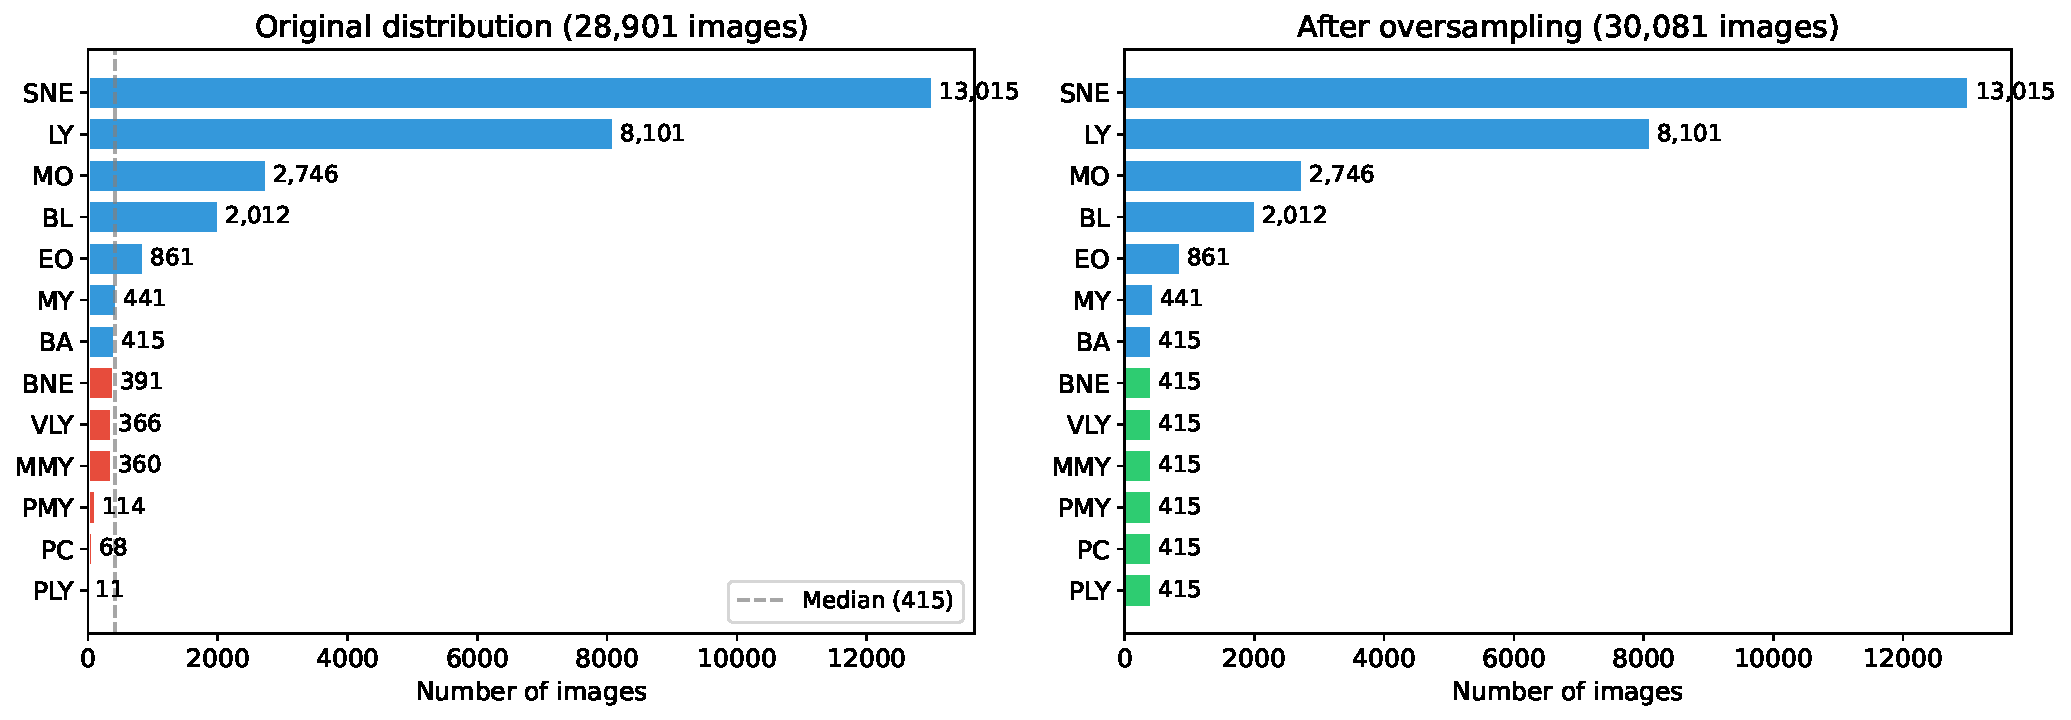
\includegraphics[width=\linewidth]{class_distribution.pdf}
    \caption{Original vs.\ oversampled class distribution. Rare classes (below median count of 415) are augmented to the median level.}
    \label{fig:class_dist}
\end{figure*}

\subsection{Visual Challenges}

Figure~\ref{fig:visual_challenges} illustrates the morphological diversity. The staining intensity varies considerably across images. Nuclear morphology---the primary discriminative feature~\cite{rezatofighi2011}---varies in shape, size, and texture across the 13 classes, but several classes share highly similar appearances (e.g., myelocyte vs.\ metamyelocyte).

\begin{figure*}[tbp]
    \centering
    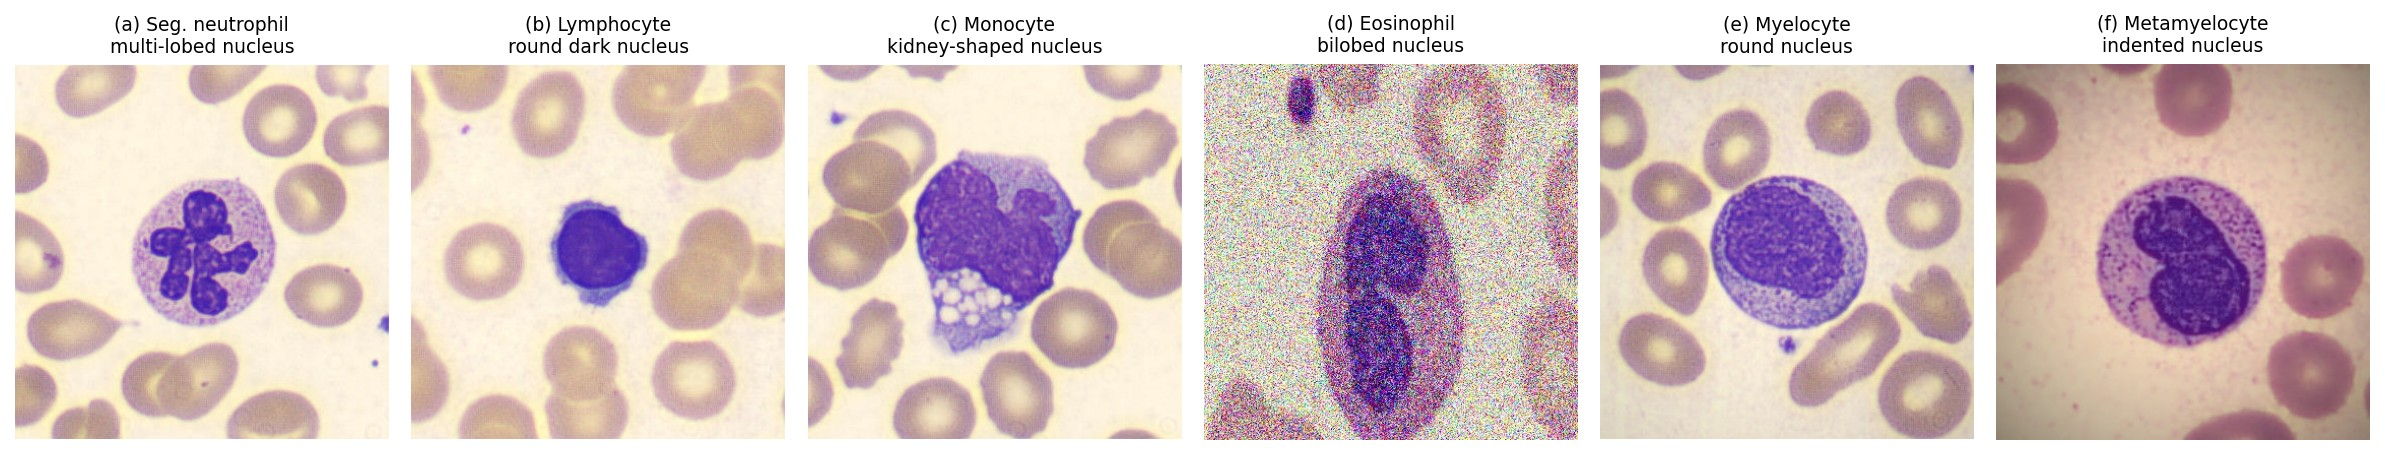
\includegraphics[width=\linewidth]{class_examples.jpg}
    \caption{Representative WBC types: (a)~Seg.\ Neutrophil, (b)~Lymphocyte, (c)~Monocyte, (d)~Eosinophil, (e)~Myelocyte, (f)~Metamyelocyte. Note the similarity between (e) and (f).}
    \label{fig:visual_challenges}
\end{figure*}


% ############################################################
% PART I --- CLASSICAL MACHINE LEARNING
% ############################################################
\section{Part I: Classical Machine Learning}

The classical approach follows the traditional pipeline recommended by Al-Dulaimi et al.~\cite{aldulaimi2018}: segmentation, feature extraction, then classification with conventional ML algorithms.

\subsection{Cell Segmentation}

Accurate separation of nucleus and cytoplasm is the critical first step, since nuclear morphology carries the strongest discriminative information. We implemented a three-stage segmentation pipeline:

\subsubsection{Reinhard Color Normalization}

Staining variability across slides causes significant color shifts that can confuse both segmentation algorithms and classifiers. We apply Reinhard color normalization~\cite{reinhard2001} in LAB color space: for each image, channel-wise mean and standard deviation are matched to a reference computed from a stratified sample of 40 images per class. This standardizes the color distribution while preserving morphological structure. \emph{Known limitation:} our implementation (\path{src/segmentation.py}) takes as reference standard deviation the spread of the per-image channel means rather than the pixel-level standard deviation, which compresses contrast before segmentation; correcting it would require re-running the whole classical pipeline.

\subsubsection{Marker-Controlled Watershed}

Cell boundary detection uses marker-controlled Watershed on the saturation channel of the HSV representation. We compute the distance transform of an initial Otsu-thresholded mask, identify foreground markers at $0.4 \times d_{\max}$ of the distance transform, and apply Watershed with these markers. The largest non-background component is selected as the cell mask.

\subsubsection{Nucleus Refinement via Geodesic Active Contours}

The nucleus is initially segmented via Otsu thresholding on the L channel (LAB) within the cell mask. This initial estimate is refined using Morphological Geodesic Active Contours (GAC) with 40 iterations, $\text{smoothing}=1$, and no balloon pressure (edge-driven only). The inverse Gaussian gradient of the L channel serves as the edge map ($\alpha=100$, $\sigma=3.0$). The cytoplasm is defined as $\text{cell} \setminus \text{nucleus}$.

\subsection{Feature Extraction}

From the segmented cell, nucleus, and cytoplasm masks, we extract a comprehensive feature vector (210 raw features) inspired by the morphological feature sets of the literature~\cite{gautam2014, aldulaimi2018}:

\begin{itemize}
    \item \textbf{Shape (A, B, D)}: Area, perimeter, circularity, eccentricity, solidity, extent, convexity, axis ratio, equivalent diameter, number of lobes, 7 Hu moments --- computed for both nucleus and cell ($\sim$25 features).

    \item \textbf{Color (C)}: Mean, std, skewness, kurtosis of each channel in RGB, HSV, and LAB color spaces, computed separately for nucleus and cytoplasm. Plus nucleus-specific ratios (R/G, R/B, G/B) ($\sim$75 features).

    \item \textbf{Texture (GLCM + LBP)}: Gray-Level Co-occurrence Matrix properties (contrast, dissimilarity, homogeneity, energy, correlation) at distances 1 and 3, angles 0, $\pi/4$, $\pi/2$. Local Binary Patterns (8 neighbors, radius 1, uniform) with 10-bin histogram. Computed for nucleus and cytoplasm ($\sim$30 features).

    \item \textbf{HOG}: Histogram of Oriented Gradients (8 orientations, 32$\times$32 pixels/cell, 2$\times$2 cells/block) on 64$\times$64 cropped regions of nucleus and cytoplasm ($\sim$64 features).

    \item \textbf{Fourier Descriptors}: 10 normalized magnitudes of the FFT of the nucleus contour, providing rotation- and scale-invariant shape encoding.
\end{itemize}

After extraction, we remove near-zero variance features (none removed: 210 remain) and features with correlation $> 0.95$ (131 remain), then add 20 PCA components (78.7\% explained variance). The final feature set contains 151 features.

\subsection{Classification}

Features are standardized (zero mean, unit variance) and class imbalance is handled via SMOTE~\cite{chawla2002smote} (k=3 neighbors) at each cross-validation fold. We evaluate 6 classifiers with 5-fold stratified cross-validation. \textbf{Computational note}: the literal SMOTE call equalizes every class up to the majority class count (SNE, 13{,}015), which would inflate each training fold to $\sim$135k rows; at that scale, the SVM-based models (SVM-RBF, Voting, Stacking) become impractically slow on 4 CPU cores. We therefore cap SMOTE oversampling at 2{,}000 samples/class (\texttt{SMOTE\_CAP} in \texttt{src/classical\_pipeline.py}) instead of equalizing to the majority class --- documented here as a deliberate adaptation for feasibility, not a change to any other part of the pipeline:

\begin{itemize}
    \item \textbf{LightGBM}~\cite{ke2017lightgbm} (hyperparameters from an earlier Optuna~\cite{akiba2019optuna} search, not included in the repository: 1755 estimators, lr=0.034, 54 leaves, depth 6)
    \item \textbf{Random Forest} (800 trees, balanced class weights)
    \item \textbf{ExtraTrees} (800 trees, balanced)
    \item \textbf{SVM-RBF} (C=10, balanced)
    \item \textbf{Soft Voting Ensemble} (LightGBM + RF + ET + SVM)
    \item \textbf{Stacking Ensemble} (same base learners, LogisticRegression meta-learner)
\end{itemize}

\subsection{Classical ML Results}

The classical ML pipeline achieves modest performance on this 13-class problem. Table~\ref{tab:classical_results} reports the 5-fold CV macro-F1 for all six classifiers (\texttt{notebooks/02\_classical\_ml.ipynb}, \texttt{results/classical\_ml/cv\_results.json}). LightGBM is the best single model; the ensembles do not improve over it under the capped-SMOTE setting.

\begin{table}[h]
\centering
\caption{Classical ML: 5-fold CV macro-F1 per classifier.}
\label{tab:classical_results}
\small
\begin{tabular}{lc}
\toprule
\textbf{Model} & \textbf{Macro-F1} \\
\midrule
LightGBM (tuned) & \textbf{0.509 $\pm$ 0.024} \\
Soft Voting & 0.496 $\pm$ 0.014 \\
Random Forest & 0.477 $\pm$ 0.018 \\
Stacking & 0.459 $\pm$ 0.018 \\
SVM-RBF & 0.444 $\pm$ 0.008 \\
ExtraTrees & 0.434 $\pm$ 0.014 \\
\bottomrule
\end{tabular}
\end{table}

OOF accuracy for the best model (LightGBM) is 0.832. The main limitations are:

\begin{enumerate}
    \item \textbf{Segmentation failures}: The Watershed+GAC pipeline fails on a non-negligible fraction of images (visual inspection: pale staining, overlapping cells, unusual backgrounds), propagating errors to all downstream features.
    \item \textbf{Feature expressiveness}: Handcrafted features cannot capture the full complexity of chromatin patterns, granule distributions, and subtle nuclear shape variations that distinguish 13 classes. Hu moments and Fourier descriptors provide rotation invariance but lose fine-grained texture.
    \item \textbf{Feature-label gap}: Features like GLCM or LBP describe texture statistically but lack the hierarchical abstraction that deep networks learn.
\end{enumerate}

These limitations motivate the transition to deep learning in Part~II.

\subsection{Feature Importance Analysis (LightGBM)}

To improve interpretability, we extracted global feature importances (split counts) from the LightGBM model trained on the full 151-feature set; the 30 top-ranked features are saved in \path{results/classical_ml/feature_importance_lightgbm.csv}. Figure~\ref{fig:feature_importance_ml} shows the top-ranked ones, and Table~\ref{tab:top10_features_ml} lists the top~10.

\begin{figure}[h]
    \centering
    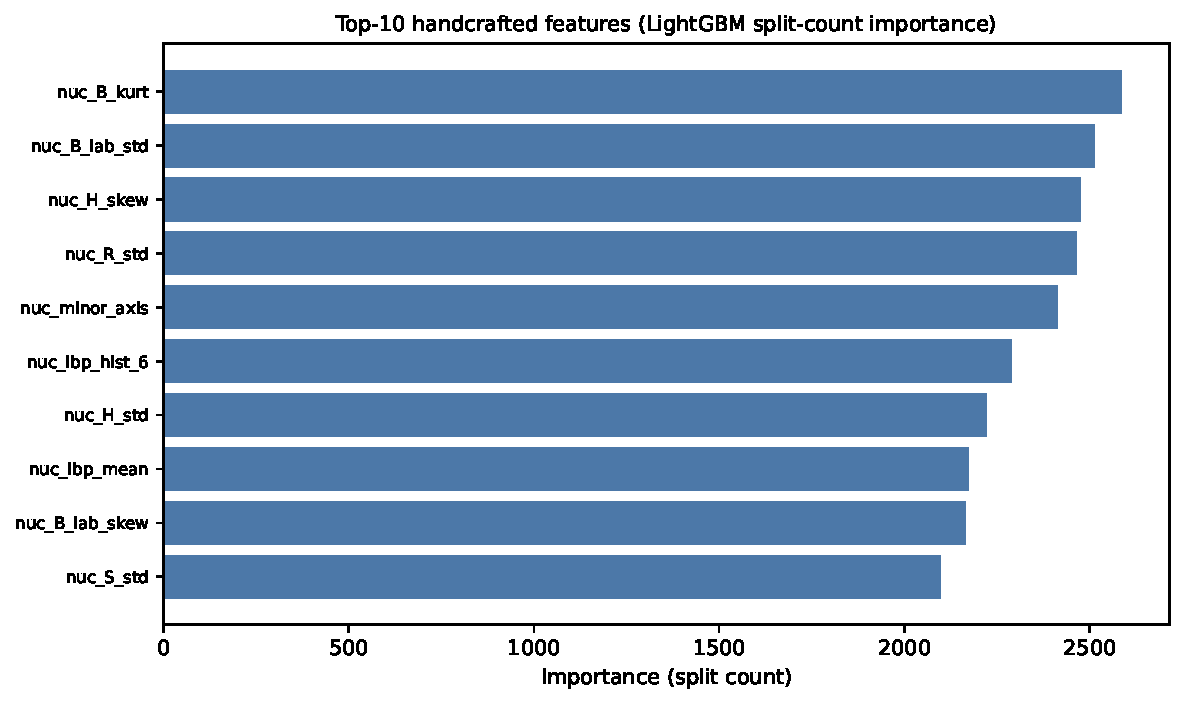
\includegraphics[width=\linewidth]{feature_importance_ml.pdf}
    \caption{Top feature importances (LightGBM split counts) in Part~I.}
    \label{fig:feature_importance_ml}
\end{figure}

\begin{table}[h]
\centering
\caption{Top-10 LightGBM features in Part~I (split-count importance). All are nucleus features.}
\label{tab:top10_features_ml}
\small
\begin{tabular}{rllr}
\toprule
\textbf{\#} & \textbf{Feature} & \textbf{Family} & \textbf{Splits} \\
\midrule
1  & \texttt{nuc\_B\_kurt}     & Color (RGB)   & 2586 \\
2  & \texttt{nuc\_B\_lab\_std} & Color (LAB)   & 2513 \\
3  & \texttt{nuc\_H\_skew}     & Color (HSV)   & 2476 \\
4  & \texttt{nuc\_R\_std}      & Color (RGB)   & 2466 \\
5  & \texttt{nuc\_minor\_axis} & Shape         & 2414 \\
6  & \texttt{nuc\_lbp\_hist\_6}& Texture (LBP) & 2289 \\
7  & \texttt{nuc\_H\_std}      & Color (HSV)   & 2221 \\
8  & \texttt{nuc\_lbp\_mean}   & Texture (LBP) & 2174 \\
9  & \texttt{nuc\_B\_lab\_skew}& Color (LAB)   & 2166 \\
10 & \texttt{nuc\_S\_std}      & Color (HSV)   & 2098 \\
\bottomrule
\end{tabular}
\end{table}

Grouping the 30 top-ranked features by family, nucleus color statistics dominate (15 features, $\approx$52\% of the top-30 split count), followed by LBP texture (5 features, $\approx$18\%), HOG (3, $\approx$8\%), shape (minor axis and area, $\approx$7\%), two PCA components ($\approx$6\%), and a single GLCM (dissimilarity), Fourier and Hu-moment feature each ($\approx$3\% each). All non-PCA features in the top~30 describe the nucleus; no cytoplasm feature appears. Notably, the classical morphometric descriptors often emphasized in the literature (circularity, eccentricity, nucleus-to-cell ratio) are \emph{not} in the top~30: the model relies mostly on higher-order color/intensity statistics and micro-texture of the nucleus, i.e.\ chromatin appearance, rather than on coarse geometry. Split-count importance is only a rough proxy (it favours continuous, frequently split features), so this ranking should be read qualitatively.


% ############################################################
% PART II --- DEEP LEARNING
% ############################################################
\section{Part II: Deep Learning}

The deep learning approach bypasses explicit segmentation and feature engineering, instead learning discriminative representations end-to-end. Our work involved \textbf{9 iterative experiments} (\texttt{deep\_1}--\texttt{deep\_9}), each addressing specific failure modes identified in the previous iteration. We first describe the deployed pipeline (\texttt{deep\_9 no-morph}, i.e.\ without handcrafted features), then detail the complete iterative journey, including \texttt{deep\_6} --- the leakage-fix milestone that established the architecture \texttt{deep\_9} refines.

\subsection{Deployed Pipeline Overview (\texorpdfstring{\texttt{deep\_9 no-morph}}{deep\_9 no-morph})}
\label{sec:deployed}

The deployed model, illustrated in Figure~\ref{fig:pipeline}, consists of six stages: (1)~cell-focused preprocessing via offline HSV-score cropping (done once), (2)~on-the-fly CLAHE on the V channel of HSV (clip limit 2.0, $8\times8$ tiles), applied to every image at train, validation and test time before augmentation, (3)~geometric and photometric augmentation (training only), (4)~a ConvNeXt-Base backbone, (5)~a lightweight SE-style channel-attention gate on the pooled features, and (6)~an MLP head, evaluated leakage-free. It is \texttt{deep\_6}'s architecture (\S\ref{sec:leakage}) plus this attention gate, the CLAHE step and a stronger augmentation; the handcrafted-morphology fusion branch that the \texttt{deep\_9} code supports is disabled here (the \texttt{no-morph} variant, see \S\ref{sec:iter_deep9}), since the ablation showed it makes no meaningful difference for this backbone.

\begin{figure*}[htbp]
\centering
\resizebox{\linewidth}{!}{%
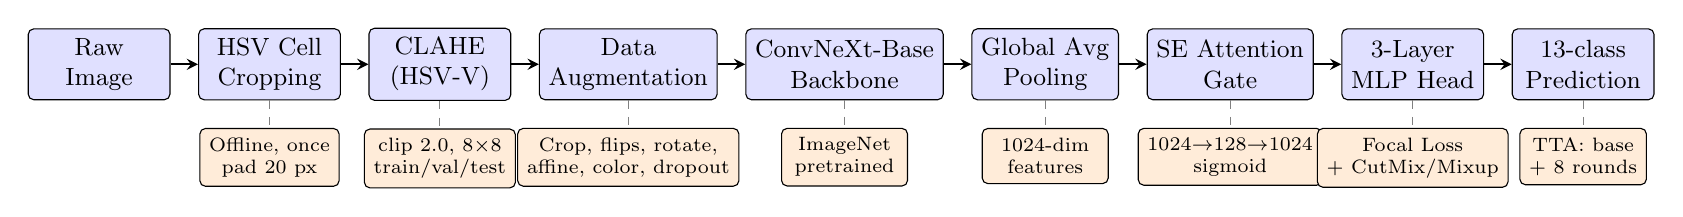
\begin{tikzpicture}[
    node distance=0.6cm and 0.35cm,
    block/.style={rectangle, draw, fill=blue!12, minimum width=1.8cm, minimum height=0.9cm, align=center, font=\small, rounded corners=2pt},
    smallblock/.style={rectangle, draw, fill=orange!15, minimum width=1.6cm, minimum height=0.7cm, align=center, font=\scriptsize, rounded corners=2pt},
    arrow/.style={thick,->,>=stealth},
]
    \node[block] (raw) {Raw\\Image};
    \node[block, right=of raw] (crop) {HSV Cell\\Cropping};
    \node[block, right=of crop] (clahe) {CLAHE\\(HSV-V)};
    \node[block, right=of clahe] (aug) {Data\\Augmentation};
    \node[block, right=of aug] (backbone) {ConvNeXt-Base\\Backbone};
    \node[block, right=of backbone] (pool) {Global Avg\\Pooling};
    \node[block, right=of pool] (gate) {SE Attention\\Gate};
    \node[block, right=of gate] (head) {3-Layer\\MLP Head};
    \node[block, right=of head] (pred) {13-class\\Prediction};

    \draw[arrow] (raw) -- (crop);
    \draw[arrow] (crop) -- (clahe);
    \draw[arrow] (clahe) -- (aug);
    \draw[arrow] (aug) -- (backbone);
    \draw[arrow] (backbone) -- (pool);
    \draw[arrow] (pool) -- (gate);
    \draw[arrow] (gate) -- (head);
    \draw[arrow] (head) -- (pred);

    \node[smallblock, below=0.35cm of crop] (hsv) {Offline, once\\pad 20 px};
    \node[smallblock, below=0.35cm of clahe] (claheD) {clip 2.0, 8$\times$8\\train/val/test};
    \node[smallblock, below=0.35cm of aug] (augd) {Crop, flips, rotate,\\affine, color, dropout};
    \node[smallblock, below=0.35cm of backbone] (bb) {ImageNet\\pretrained};
    \node[smallblock, below=0.35cm of pool] (poold) {1024-dim\\features};
    \node[smallblock, below=0.35cm of gate] (gated) {1024$\to$128$\to$1024\\sigmoid};
    \node[smallblock, below=0.35cm of head] (hd) {Focal Loss\\+ CutMix/Mixup};
    \node[smallblock, below=0.35cm of pred] (tta) {TTA: base\\+ 8 rounds};

    \draw[-,dashed,gray] (crop) -- (hsv);
    \draw[-,dashed,gray] (clahe) -- (claheD);
    \draw[-,dashed,gray] (aug) -- (augd);
    \draw[-,dashed,gray] (backbone) -- (bb);
    \draw[-,dashed,gray] (pool) -- (poold);
    \draw[-,dashed,gray] (gate) -- (gated);
    \draw[-,dashed,gray] (head) -- (hd);
    \draw[-,dashed,gray] (pred) -- (tta);
\end{tikzpicture}}
\caption{Deep learning pipeline (\texttt{deep\_9 no-morph}). Offline HSV cropping removes background distractors, CLAHE on the HSV V channel equalizes local contrast (at train, validation and test time), augmentation builds geometric and photometric robustness (training only), ConvNeXt-Base learns hierarchical features, an SE-style gate reweights channels, and Focal Loss handles class imbalance. The handcrafted-morphology fusion branch this architecture supports is present in code but disabled in this \texttt{no-morph} variant.}
\label{fig:pipeline}
\end{figure*}

\subsection{Preprocessing: HSV-Based Cell Cropping and CLAHE}

Unlike the classical approach which requires precise nucleus/cytoplasm segmentation, the DL approach only needs a coarse cell crop to remove background clutter. We designed an HSV-based algorithm that scores each pixel:
\[
S(x,y) = 0.55 \cdot H_s + 0.25 \cdot S_s + 0.20 \cdot V_s
\]
where $H_s$ measures proximity to hue $\approx 140$ (purple), $S_s$ measures saturation, and $V_s$ penalizes bright pixels. After thresholding at the 92nd percentile, morphological cleanup, and selection of the largest connected component near the image center, the mask is dilated with a $45\times45$ elliptical kernel and the bounding box (with 20px padding) defines the crop.

This preprocessing is performed \textbf{once, offline}, and saved to disk, which removes the runtime cropping bottleneck of the earlier iterations; crop quality was checked visually (\texttt{deep\_6} QC, \S\ref{sec:leakage}). With offline crops, the deployed model trains at $\approx$84\,s/epoch (frozen backbone) and $\approx$140\,s/epoch (fine-tuning) on a single RTX~3090.

On top of the stored crops, \texttt{deep\_9} applies CLAHE (contrast-limited adaptive histogram equalization) to the V channel of the HSV representation (clip limit 2.0, $8\times8$ tiles) on the fly. This step is deterministic and applied to every image at train, validation and test time, \emph{before} augmentation; hue and saturation are left unchanged.

\begin{figure}[h]
    \centering
    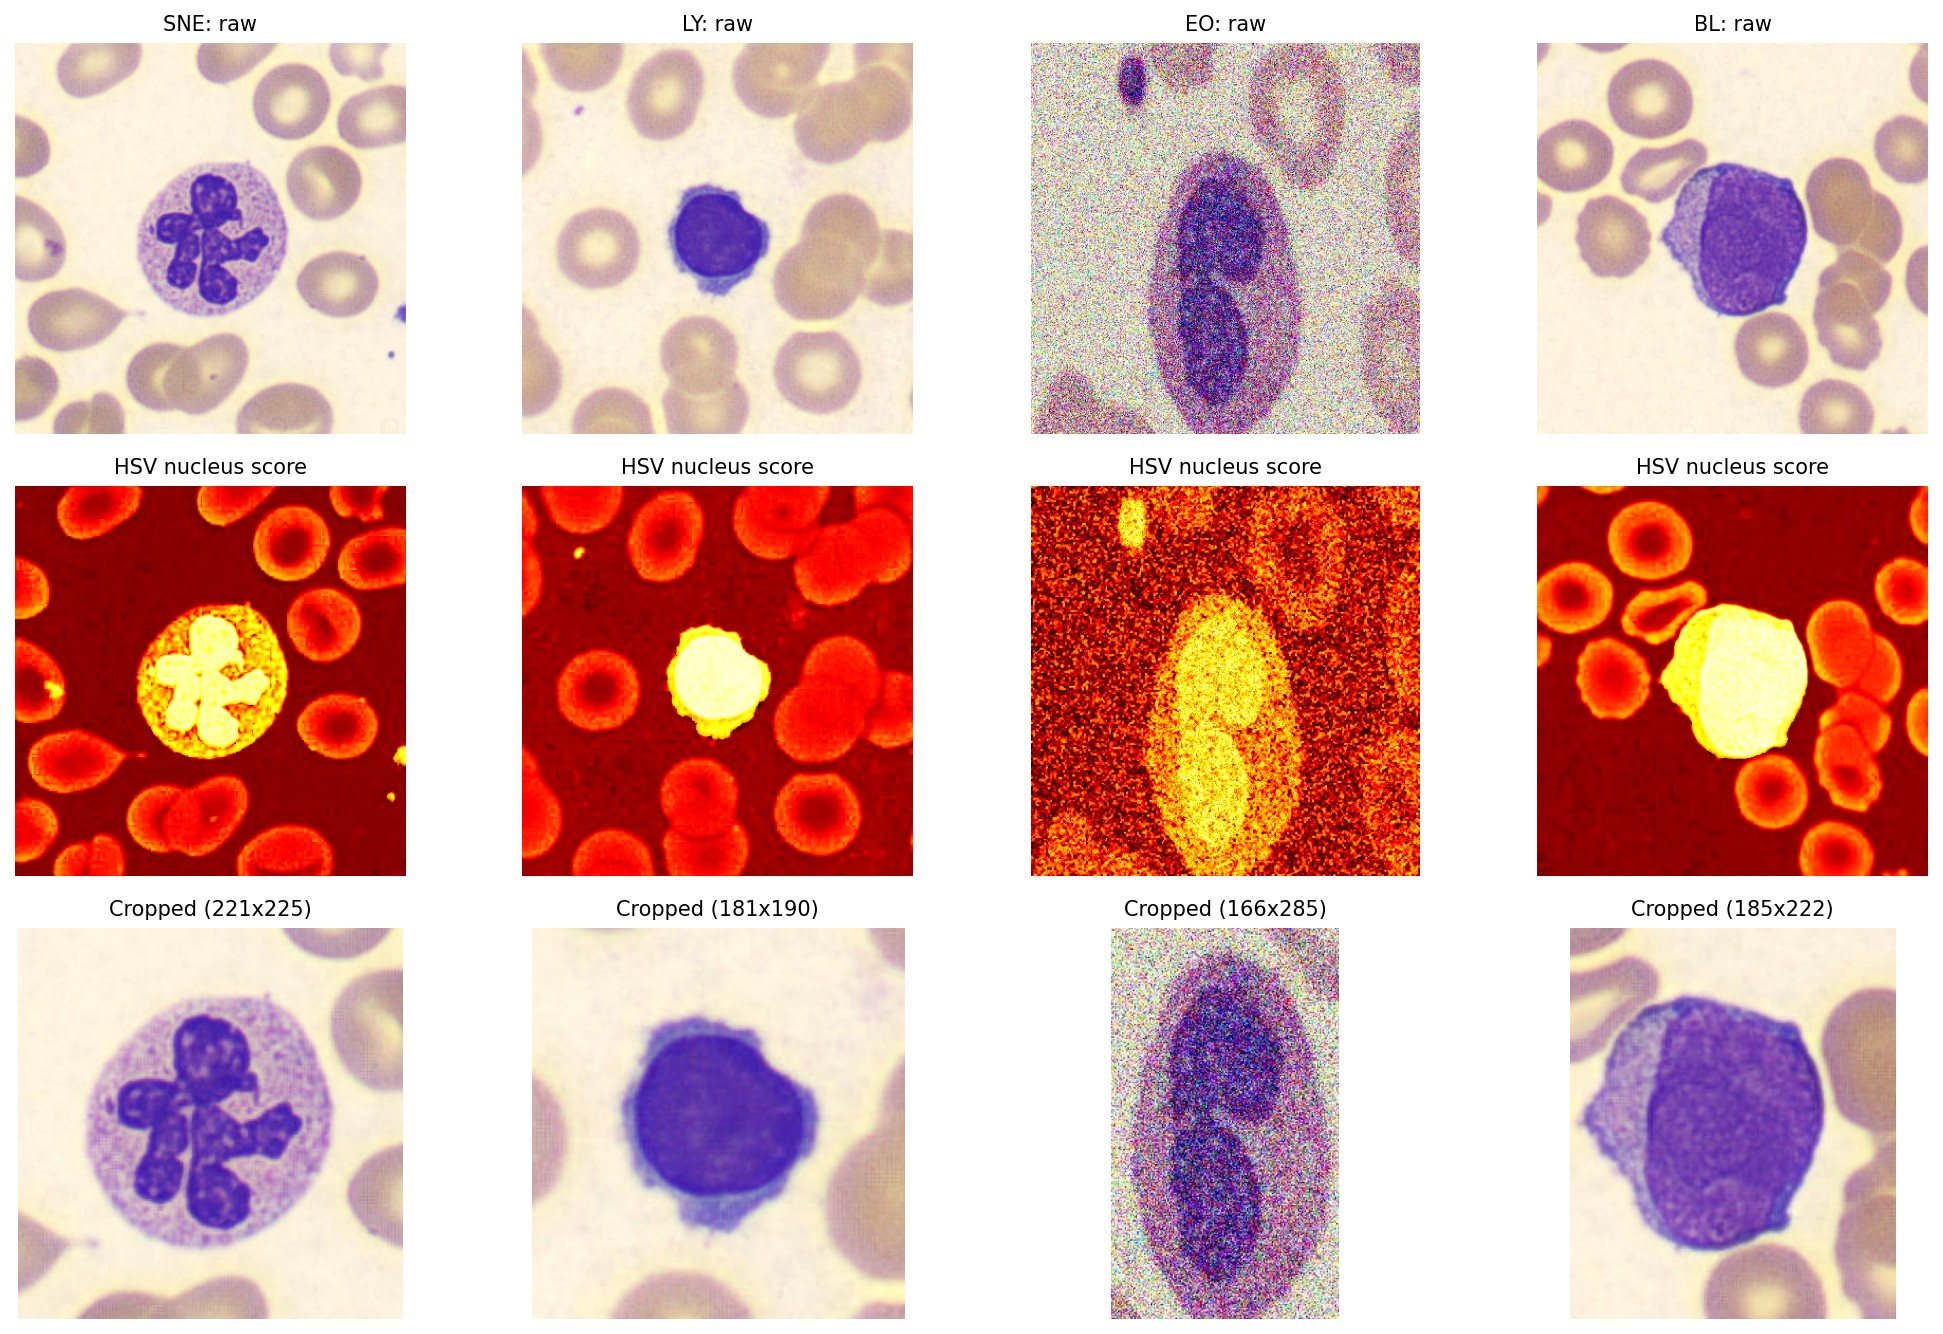
\includegraphics[width=\linewidth]{crop_examples.jpg}
    \caption{HSV-based cell cropping. Top: raw images. Middle: HSV score heatmaps. Bottom: cropped outputs.}
    \label{fig:crop_examples}
\end{figure}

\subsection{Handling Class Imbalance}

We combine three strategies:
\begin{enumerate}
    \item \textbf{Offline oversampling}: The 6 rarest classes (below median count 415) are augmented to 415 images each with random flips, rotations, translations, brightness/contrast changes and Gaussian noise.
    \item \textbf{WeightedRandomSampler}: Sampling weights proportional to $n_c^{-1/2}$ (inverse square root of the class count) balance batch composition during training.
    \item \textbf{Focal Loss}~\cite{lin2017focal}: $\mathcal{L}_{\text{FL}} = -(1 - p_t)^\gamma \log(p_t)$ with $\gamma=2.0$, combined with label smoothing~\cite{szegedy2016rethinking} ($\epsilon=0.05$), down-weighting easy/common examples.
\end{enumerate}

\textbf{Data leakage prevention}: Augmented copies must stay in the same split as their parent. An earlier iteration (\texttt{deep\_5}) that split \textit{after} augmentation inflated F1 from 0.70 to 0.82. We fixed this in \texttt{deep\_6} by splitting only original images, then assigning augmented copies to their parent's split (see Section~\ref{sec:leakage}).

\subsection{Data Augmentation}

The training-time augmentation of the deployed model (\texttt{deep\_9 no-morph}) uses Albumentations~\cite{buslaev2020} with geometric transforms and moderate photometric perturbation (Table~\ref{tab:augmentation}); validation and test images are only resized to $224\times224$ and normalized.

\begin{table}[h]
\centering
\caption{Training augmentation of \texttt{deep\_9 no-morph} (applied after CLAHE, in this order).}
\label{tab:augmentation}
\footnotesize
\setlength{\tabcolsep}{3pt}
\begin{tabular}{@{}>{\raggedright\arraybackslash}p{4.1cm}>{\raggedright\arraybackslash}p{0.75cm}>{\raggedright\arraybackslash}p{3.15cm}@{}}
\toprule
\textbf{Transform} & \textbf{Prob.} & \textbf{Challenge Addressed} \\
\midrule
RandomResizedCrop(224, scale 0.75--1.0, ratio 0.9--1.1) & 0.7 & Scale/position variation \\
Horizontal flip, vertical flip, RandomRotate90 & 0.5 each & Arbitrary orientation \\
Rotate($\pm180^{\circ}$) & 0.9 & Full 360$^{\circ}$ coverage \\
Affine (translate $\pm$10\%, scale 0.85--1.15, shear $\pm8^{\circ}$) & 0.5 & Geometric robustness \\
ColorJitter (B 0.3, C 0.3, S 0.2, H 0.03) & 0.7 & Brightness/contrast/stain var.\ \\
ToGray & 0.2 & Reliance on shape over color \\
One of GaussianBlur / GaussNoise & 0.2 & Acquisition artifacts \\
Resize($224\times224$) + ImageNet normalize & 1.0 & Uniform input \\
CoarseDropout (1--3 holes, 16--32\,px) & 0.25 & Occlusion robustness \\
\bottomrule
\end{tabular}
\end{table}

\textbf{Note}: Apart from the small hue jitter in ColorJitter, this pipeline does \textit{not} include explicit stain-specific augmentation (HSV shifts, RGBShift); these were used in \texttt{deep\_2}. CLAHE is not an augmentation here but a deterministic preprocessing step shared by training and inference.

\begin{figure}[h]
    \centering
    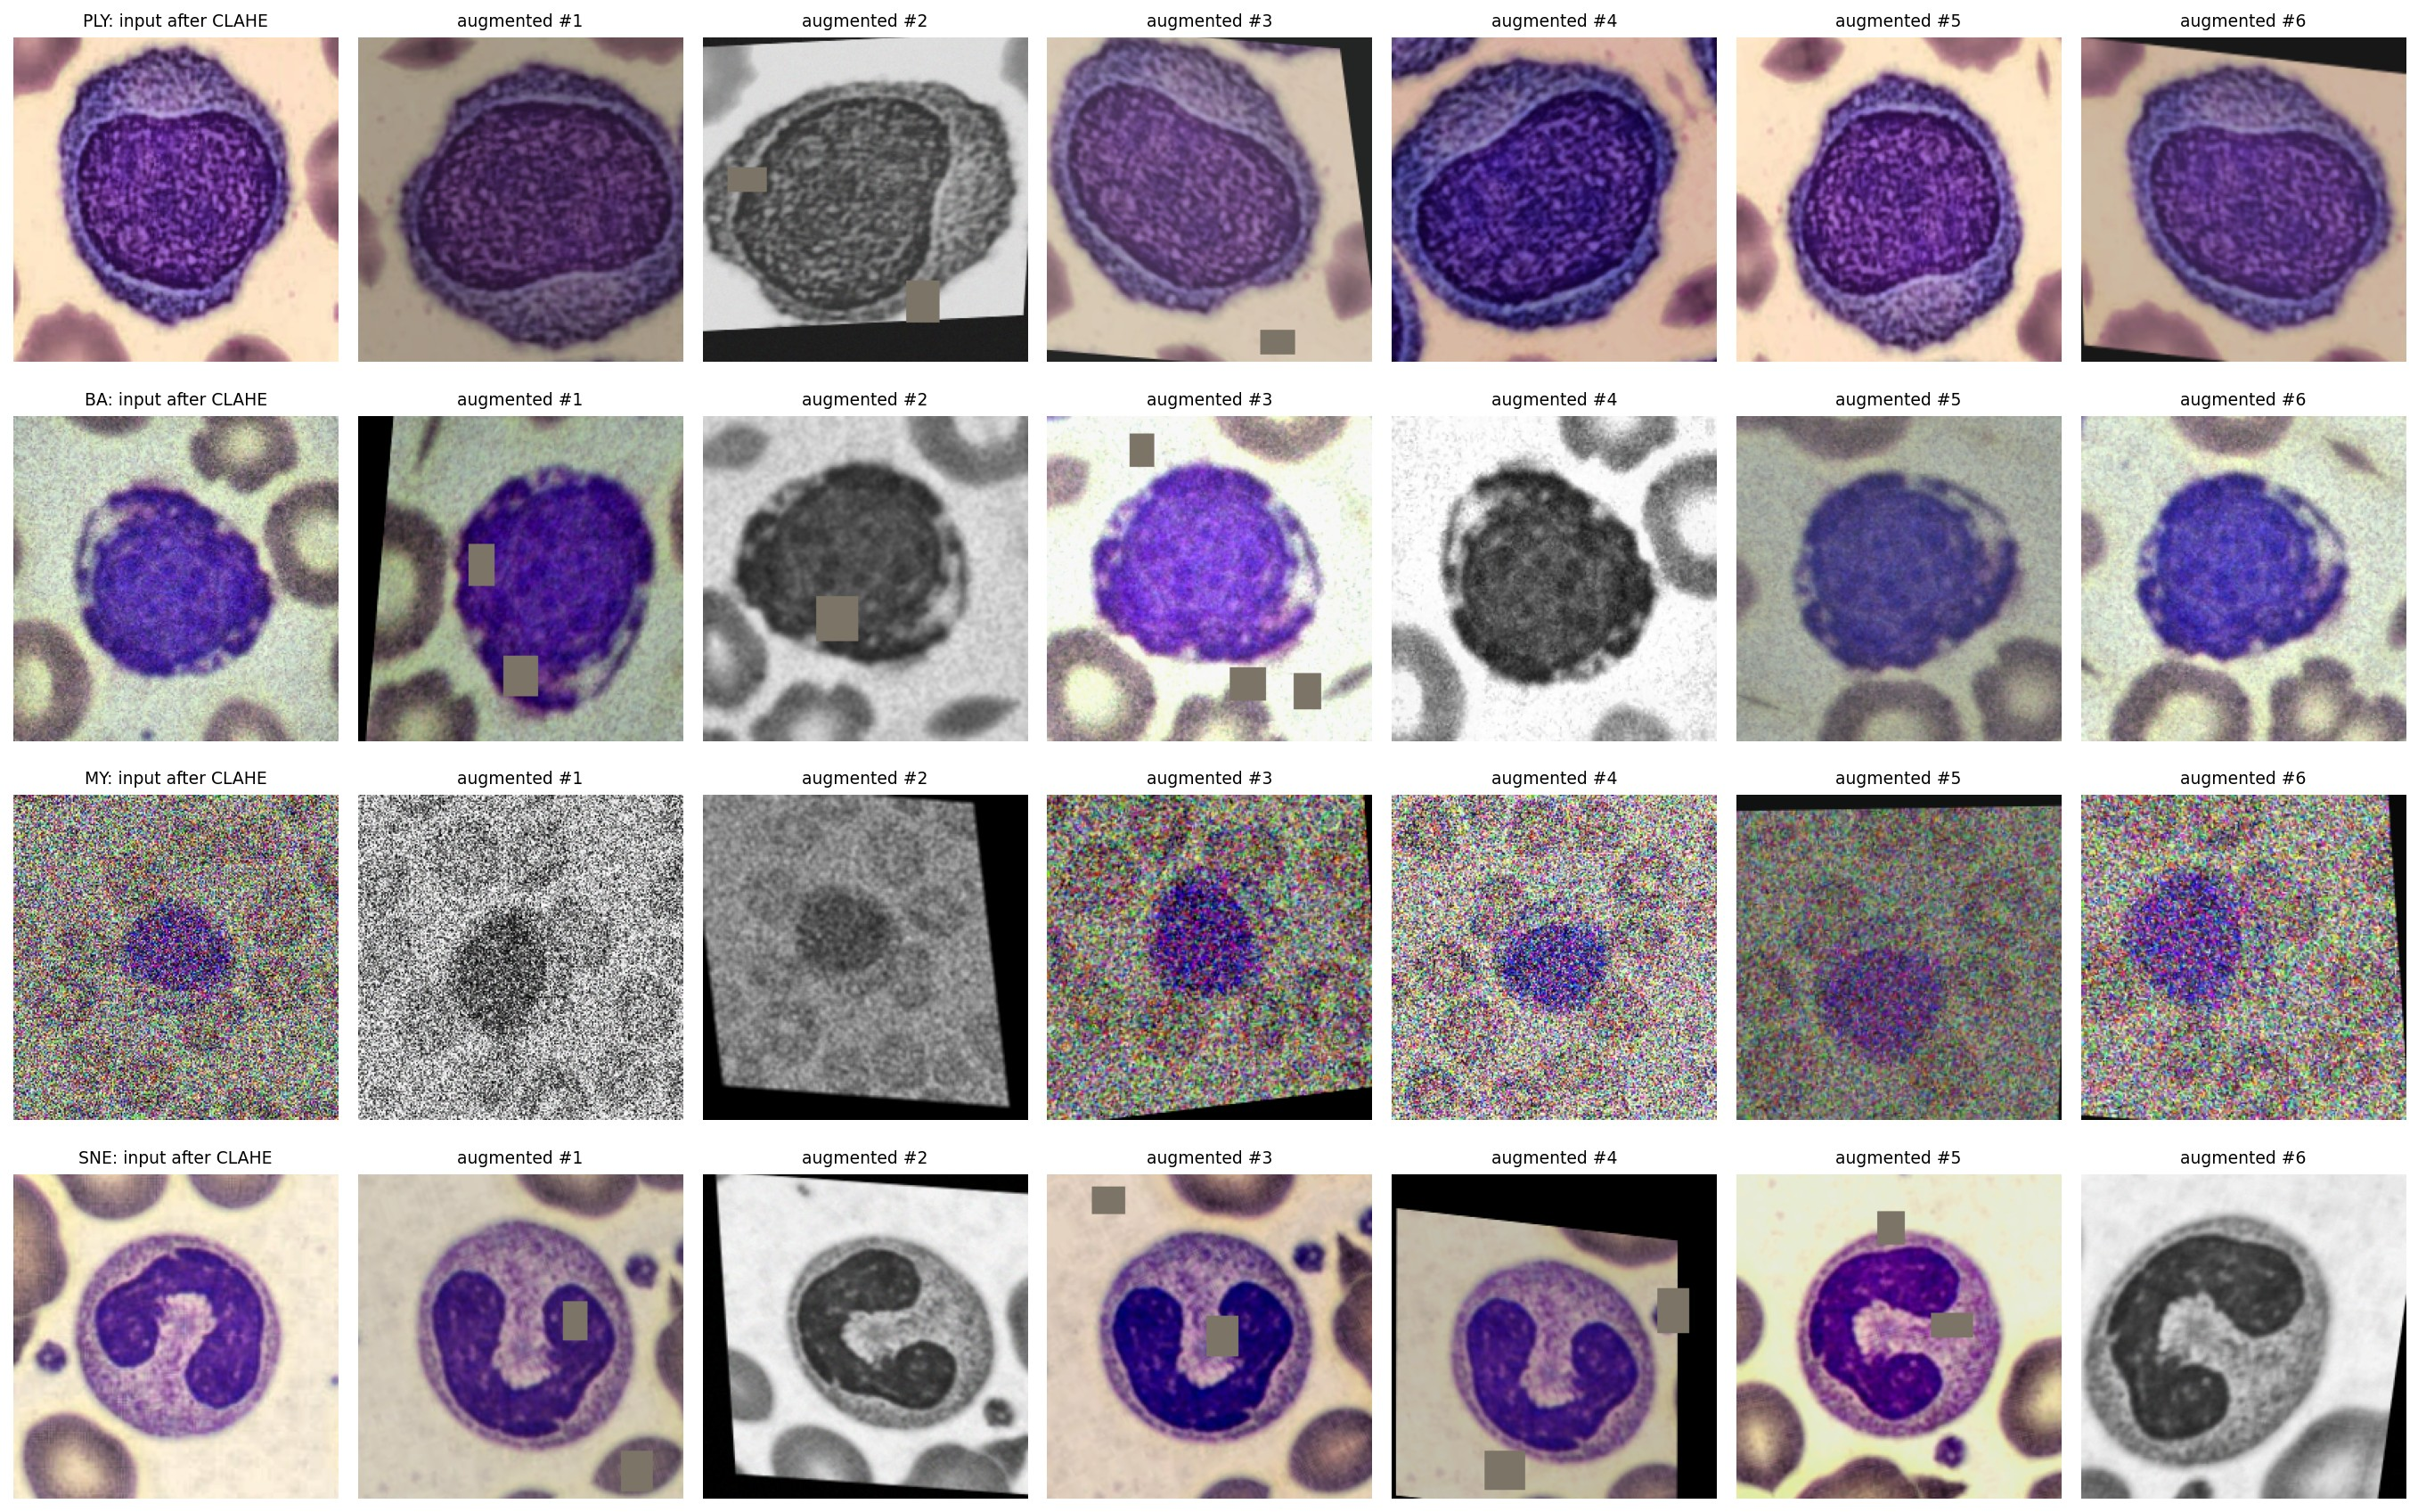
\includegraphics[width=\linewidth]{augmentation_gallery.jpg}
    \caption{Training-time augmentation of the deployed model (\texttt{deep\_9 no-morph}): CLAHE-processed crop (left) and augmented views drawn from the actual training pipeline (CLAHE followed by the transforms of Table~\ref{tab:augmentation}).}
    \label{fig:augmentation_gallery}
\end{figure}

\subsection{Architecture: ConvNeXt-Base + SE Gate + MLP Head}

\subsubsection{Transfer Learning with ConvNeXt}

Al-Dulaimi et al.~\cite{aldulaimi2018} warn that training deep networks from scratch requires datasets far larger than typical medical imaging datasets. Following this guidance, we use transfer learning with ConvNeXt-Base~\cite{liu2022convnext} (torchvision, pre-trained on ImageNet; 87.6M backbone parameters), which modernizes the CNN architecture with design elements from Vision Transformers while retaining CNN efficiency. Our architecture choice evolved from EfficientNet-B3 (12M params, single-split F1 = 0.552) to ConvNeXt-Base (val F1 = 0.70+). The comparison with the similarly sized ResNeXt101 (\texttt{deep\_8}, \S\ref{sec:iter_deep8}) suggests that model size alone does not explain this gain, although \texttt{deep\_8} also differs from \texttt{deep\_6} in several other respects.

\subsubsection{Channel-Attention Gate and Classification Head}

After global average pooling, the 1024-dimensional feature vector passes through a lightweight SE-style~\cite{hu2018squeeze} channel-attention gate ($1024 \to 128 \to 1024$, sigmoid, 263,296 params) that reweights features before the head, then a 3-layer MLP: $1024 \to 512 \to 256 \to 13$ with ReLU and dropout ($p=0.3$; 659,469 params). The full model has 88,487,181 parameters (backbone 87,564,416). Heavier attention mechanisms (CBAM, spatial attention) and handcrafted feature branches were also tried (Sections~\ref{sec:iter_deep7}--\ref{sec:iter_deep9}) and provided negligible-to-no gains; \texttt{deep\_9} (SE gate, CLAHE and stronger augmentation) scores 0.7052 against 0.6994 for \texttt{deep\_6}, a difference within the noise of a single validation split (\S\ref{sec:eval}). The architecture otherwise remains deliberately simple---no CBAM, no spatial attention, no multi-task heads.

\subsection{Training Strategy}

\subsubsection{Two-Phase Training}

\begin{enumerate}
    \item \textbf{Phase 1 -- Warmup} (epochs 1--5): Backbone \textit{frozen}; only the SE gate and MLP head are trained (922,765 trainable params: gate 263K + head 659K), AdamW~\cite{loshchilov2019decoupled}, lr=$3\times10^{-4}$, cosine annealing with warm restarts.
    \item \textbf{Phase 2 -- Fine-tuning} (up to epoch 60): Backbone \textit{unfrozen}; AdamW with the \emph{same} learning rate $10^{-4}$ for backbone and head (no differential learning rate), weight decay $10^{-4}$.
\end{enumerate}

Early stopping (patience=10 on val macro-F1) prevents overfitting. Training uses batch size 16 with 4-step gradient accumulation (effective=64), AMP fp16 mixed precision, and gradient clipping at norm 1.0. The best validation macro-F1 (0.7052) was reached at epoch 21, and training stopped early at epoch 31.

\subsubsection{Final Hyperparameters (\texorpdfstring{\texttt{deep\_9 no-morph}}{deep\_9 no-morph})}

For reproducibility, Table~\ref{tab:deep9_hparams} consolidates the training configuration used for the deployed model. The figure-generation scripts and the notebooks expect the Kaggle challenge data to be placed in \texttt{data/}; the data itself is not versioned in the repository.

\begin{table}[h]
\centering
\caption{Final hyperparameters for \texttt{deep\_9 no-morph}.}
\label{tab:deep9_hparams}
\footnotesize
\setlength{\tabcolsep}{4pt}
\begin{tabular}{@{}>{\raggedright\arraybackslash}p{2.5cm}>{\raggedright\arraybackslash}p{5.6cm}@{}}
\toprule
\textbf{Parameter} & \textbf{Value} \\
\midrule
Backbone & ConvNeXt-Base (torchvision, ImageNet) \\
Attention & SE-style channel gate (1024$\to$128$\to$1024, sigmoid) \\
Head & MLP 1024$\to$512$\to$256$\to$13, ReLU, dropout 0.3 \\
Parameters & 88.49M total; 0.92M trainable in phase 1 \\
Preprocessing & Offline HSV crop (pad 20) + CLAHE on HSV-V (clip 2.0, 8$\times$8), train/val/test \\
Split & 90/10 stratified on original images (seed 42); 27,081 train / 2,891 val \\
Sampler & WeightedRandomSampler, weights $\propto n_c^{-1/2}$ \\
Optimizer & AdamW~\cite{loshchilov2019decoupled} \\
Phase-1 LR (gate + head) & $3\times10^{-4}$, cosine warm restarts, 5 epochs \\
Phase-2 LR (all) & $1\times10^{-4}$ (backbone and head, same LR) \\
Weight decay & $1\times10^{-4}$ \\
Batch size & 16 $\times$ 4 accumulation steps (effective 64) \\
Epoch budget & 60 max; best epoch 21, early stop at 31 \\
Early stopping & Patience 10 (val macro-F1) \\
Loss & Focal Loss ($\gamma=2.0$) + label smoothing ($\epsilon=0.05$) \\
Batch mixing & CutMix ($\alpha=1.0$, $p=0.5$) / Mixup ($\alpha=0.2$); off for batches with rare classes \\
Precision & AMP fp16 \\
Gradient clipping & Norm 1.0 \\
Input resolution & $224\times224$ \\
TTA & Base pass + 8 stochastic rounds (H/V flip, rot90), logits averaged \\
Hardware & 1$\times$ RTX 3090; $\approx$84\,s / $\approx$140\,s per epoch (frozen / fine-tune) \\
\bottomrule
\end{tabular}
\end{table}

\subsubsection{CutMix and Mixup}

CutMix~\cite{yun2019cutmix} ($\alpha=1.0$) and Mixup~\cite{zhang2018mixup} ($\alpha=0.2$) are applied as batch-level augmentations, CutMix being chosen with probability 0.5 and Mixup otherwise. \textbf{Crucially}, both are \textit{disabled} for batches containing rare class samples to avoid diluting their scarce training signal.

\subsection{Evaluation Protocol}
\label{sec:eval}

\begin{itemize}
    \item \textbf{Leakage-free split}: 90\%/10\% stratified train/val split on original images only (seed 42). Augmented copies follow their parent's split. Validation contains originals only (27,081 train / 2,891 val).
    \item \textbf{Macro-F1} as primary metric (same as Kaggle leaderboard).
    \item \textbf{Test inference}: CLAHE-preprocessed crops, one base pass plus 8 stochastic TTA rounds (random H/V flips and 90$^\circ$ rotations), with logits averaged.
\end{itemize}

\textbf{Limitations of the validation score.} The same 2,891 validation images are used for early stopping, for choosing between end-to-end and hybrid classifiers, and for comparing iterations, so the reported validation scores are somewhat optimistic and are not an independent test score. They come from a single split and a single training seed; with 1 PLY and 7 PC images in validation, one prediction can move the macro-F1 by several points (a single PLY image changes it by about 0.077), so differences below about 0.01 between iterations are not meaningful.


% ============================================================
\section{Iterative Development: The Full Journey}
\label{sec:iterations}
% ============================================================

A key aspect of this work was iterative refinement across 9 experiments. Each iteration addressed specific failure modes identified in the previous one. Table~\ref{tab:iterations} summarizes all experiments, and the following subsections detail each.

\begin{table*}[t]
\centering
\caption{Summary of all deep learning iterations. F1 = validation macro-F1. ``Best approach'' indicates whether end-to-end DL or a hybrid (backbone features fed to RF/SVM) performed better.}
\label{tab:iterations}
\footnotesize
\setlength{\tabcolsep}{4pt}
\begin{tabular}{@{}ll>{\raggedright\arraybackslash}p{4.4cm}cc>{\raggedright\arraybackslash}p{4.6cm}@{}}
\toprule
\textbf{Iter.} & \textbf{Backbone} & \textbf{Key Innovation} & \textbf{Best F1} & \textbf{Best Approach} & \textbf{Key Finding} \\
\midrule
\texttt{deep\_1} & EfficientNet-B3 & Baseline, weighted CE & 0.552$^\dagger$ & DL & Established initial baseline \\
\texttt{deep\_2} & EffNet-B3 + CBAM & HSV crop, Albumentations, hybrid & 0.633 & CNN+SVM & SVM on CNN features $>$ DL \\
\texttt{deep\_3} & EffNet-B3 + CBAM & Late fusion, Wiener/Laplacian, RGBM & 0.641 & Fused+SVM & Marginal gain from fusion \\
\texttt{deep\_4} & EffNet-B3 + CBAM & Gautam 2014 segmentation, 4 feats & 0.591 & Fused+RF & Rigid pipeline \textit{hurt} perf.\ \\
\texttt{deep\_5} & ConvNeXt-Base & Focal Loss, CutMix, 2-phase, offline & 0.822 & DL & \textbf{Inflated by data leakage!} \\
\texttt{deep\_6} & ConvNeXt-Base & Leakage fix, visual QC & 0.699 & DL & True performance after leakage fix \\
\texttt{deep\_7} & ResNet50 + SpatialAtt & Late fusion, 4 morpho feats & 0.651 & DL & Weaker backbone $\Rightarrow$ lower F1 \\
\texttt{deep\_8} & ResNeXt101 + CBAM & Multi-task aux heads, 6 morpho feats & 0.665 & DL & Complex but no gain over \texttt{deep\_6} \\
\texttt{deep\_9} & ConvNeXt + SE & SE gate, HSV-V CLAHE, with-/no-morph ablation & \textbf{0.705} & DL & \textbf{Deployed model}; morpho feats $\approx$ no effect \\
\bottomrule
\end{tabular}

\vspace{2pt}
{\footnotesize $^\dagger$\texttt{deep\_1}'s original run (5-fold CV, up to 30 epochs/fold) has no saved outputs in the source notebook and could not be verified; 0.552 is from a seeded re-run (\path{scripts/deep_1_rerun.py}) under a reduced protocol (single stratified 85/15 split, 15-epoch cap) kept within a practical compute budget -- see \S\ref{sec:iter_deep1}. It is not directly comparable to the other rows' full training budgets. Validation sets differ: \texttt{deep\_2}--\texttt{deep\_4} use a single 85/15 split (4,336 images), \texttt{deep\_5} split after oversampling (leaky), and \texttt{deep\_6}--\texttt{deep\_9} share the same leakage-free 90/10 split (2,891 original images). For \texttt{deep\_2}--\texttt{deep\_4}, ``Best F1'' is the best of the end-to-end and hybrid classifiers, selected on this validation set.}
\end{table*}

\subsection{\texorpdfstring{\texttt{deep\_1}}{deep\_1}: EfficientNet-B3 Baseline}
\label{sec:iter_deep1}

The first deep learning attempt used EfficientNet-B3~\cite{tan2019efficientnet} (12M parameters, ImageNet pretrained) with a simple classifier head (Dropout(0.4) + Linear), torchvision transforms (basic flips, rotation, color jitter), WeightedRandomSampler, and weighted CrossEntropyLoss, originally run with 5-fold stratified K-Fold cross-validation and three TTA variants (original, H-flip, V-flip) at inference.

\textbf{Note}: the original 5-fold run was saved without outputs, so its score cannot be checked. The same model, loss and sampler were therefore re-run under a shorter protocol (a single stratified 85/15 split, at most 15 epochs instead of up to 30 per fold $\times$ 5 folds); the numbers above come from this re-run (\path{results/deep_1_rerun/}).

\textbf{Results (re-run)}: val macro-F1 = 0.552, accuracy = 0.716. Per-class F1: BA=0.92, BL=0.83, LY=0.82, SNE=0.81, MO=0.79, EO=0.78, MY=0.52, PMY=0.40, PC=0.34, MMY=0.30, VLY=0.27, PLY=0.25, BNE=0.14. This score is noisy: the validation macro-F1 still oscillated between 0.44 and 0.55 over the last epochs, and an earlier unseeded run of the same script reached 0.489. Even undertrained, transfer learning is already on par with the classical pipeline (0.509, under a different protocol), with rare classes remaining the main weakness -- a pattern that persists across every later iteration.

\subsection{\texorpdfstring{\texttt{deep\_2}}{deep\_2}: CBAM Attention + Nucleus Cropping}

\textbf{Motivation}: Improve focus on the nucleus (the primary discriminative feature) and add domain-specific augmentation.

\textbf{Changes}: Switched to the \texttt{timm} library for feature extraction with Spatial CBAM~\cite{woo2018cbam} (channel + spatial attention) on the last feature map. Added HSV-based nucleus cropping at runtime and a comprehensive Albumentations~\cite{buslaev2020} pipeline including staining variation (HSV shifts, RGBShift, CLAHE). Introduced label smoothing~\cite{szegedy2016rethinking} (0.1), Mixup ($\alpha$=0.4), gradient clipping, and CosineAnnealingWarmRestarts. Tested CNN+RF and CNN+SVM hybrids on extracted backbone features. Used a single 85/15 split for faster iteration.

\textbf{Results}: DL-only macro-F1 = 0.552, but CNN+SVM achieved \textbf{0.633}---a significant finding that SVM on CNN features substantially outperformed end-to-end training with the small EfficientNet backbone. Training was slow because HSV cropping was still performed at runtime. Per-class: SNE=0.96, LY=0.94, but PLY=0.00, PMY=0.22, BNE=0.31.

\textbf{Key insight}: For smaller backbones, the learned representation benefits from a classical classifier (SVM/RF) rather than the trained softmax head.

\subsection{\texorpdfstring{\texttt{deep\_3}}{deep\_3}: Late Fusion + Wiener/Laplacian + 4th Channel}

\textbf{Motivation}: Inject explicit morphological knowledge that the CNN might miss, inspired by classical segmentation literature~\cite{rezatofighi2011}.

\textbf{Changes}: Two-branch Late Fusion model: (1)~EfficientNet-B3 + CBAM with 4-channel input (RGB + nucleus mask as 4th channel), (2)~MLP on 8 handcrafted morphometry features (roundness, solidity, compactness, eccentricity, C/N ratio, normalized area, perimeter, extent). Added Wiener filter denoising and Laplacian edge enhancement as preprocessing. Mixup applied to both branches with consistent $\lambda$/permutation.

\textbf{Results}: DL-only F1 = 0.552, Fused+SVM = \textbf{0.641}---a marginal +0.8pp over \texttt{deep\_2}. The additional complexity (4th channel, Wiener filtering) did not translate into meaningful gains for the DL head. Training became considerably slower because of the Wiener filtering, while macro-F1 was nearly unchanged.

\textbf{Key insight}: Adding complexity to the input (4th channel, denoising filters) increases computational cost without proportional performance gains.

\subsection{\texorpdfstring{\texttt{deep\_4}}{deep\_4}: Literature Segmentation Pipeline (Failed Experiment)}

\textbf{Motivation}: Replace our ad-hoc nucleus segmentation with the published pipeline of Gautam and Bhadauria~\cite{gautam2014} (contrast stretch + histogram equalization + add/subtract isolation + minimum filter + Otsu + morphological closing + border clearing).

\textbf{Changes}: Adopted the paper's exact segmentation pipeline. Reduced handcrafted features from 8 to 4 (area, perimeter, eccentricity, circularity). Removed class weights from the loss function (only WeightedRandomSampler) to fix NaN gradient explosions caused by double imbalance correction. Added NaN guards (torch.nan\_to\_num on inputs, skip NaN-loss batches).

\textbf{Results}: Performance \textit{dropped} to F1 = \textbf{0.591}. Per-class: SNE=0.95, LY=0.90, but BNE=0.24, PMY=0.27, PC=0.33---a clear regression in macro-F1 from \texttt{deep\_3} (0.641 $\to$ 0.591), driven by the rare classes.

\textbf{Key insight}: Classical segmentation pipelines designed for clean laboratory conditions do not generalize to heterogeneous real-world staining. This failure strongly motivated abandoning complex feature engineering in favor of end-to-end learning.

\subsection{\texorpdfstring{\texttt{deep\_5}}{deep\_5}: The ConvNeXt Pivot + Data Leakage Discovery}

\textbf{Motivation}: After diminishing returns from complex feature engineering (\texttt{deep\_2}--\texttt{deep\_4}, all in the 0.55--0.64 range), try a fundamentally stronger backbone with a simpler pipeline.

\textbf{Changes}: Complete pipeline redesign---removed all attention modules, handcrafted features, and mask channels. ConvNeXt-Base~\cite{liu2022convnext} (88M params, $\sim$7$\times$ larger than EfficientNet-B3), 3-layer MLP head, Focal Loss~\cite{lin2017focal} ($\gamma$=2.0), CutMix~\cite{yun2019cutmix}+Mixup~\cite{zhang2018mixup} (disabled for rare classes), 2-phase training (warmup then finetune), AMP mixed precision, gradient accumulation, offline oversampling of rare classes to median count, offline HSV pre-cropping (removing the runtime cropping bottleneck), stochastic TTA (8 rounds).

\textbf{Results}: Achieved validation F1 = \textbf{0.822}---a massive jump from the best previous result (0.641). \textit{However, this was inflated by data leakage.}

\textbf{The leakage}: Augmented copies of images were split \textit{after} augmentation, meaning an augmented copy of image X could appear in validation while the original X was in training. The model effectively memorized these images.

\subsection{\texorpdfstring{\texttt{deep\_6}}{deep\_6}: Leakage Fix --- True Performance}
\label{sec:leakage}

\textbf{Motivation}: Eliminate data leakage and measure true generalization.

\textbf{Changes}: Split on \textit{original} image identity before assigning augmented copies. Validation set contains only original images (no augmented copies). Added comprehensive visual QC: raw vs.\ cropped comparison per class, crop size distributions, failure detection (crops covering $>$90\% of original area), train vs.\ test crop ratio comparison.

\textbf{Results}: True macro-F1 = 0.6994, accuracy = 0.936. The 12.3-point absolute drop from \texttt{deep\_5} (0.822 $\to$ 0.699, $\approx$15\% relative) demonstrates the severity of the leakage. A hybrid approach (backbone features $\to$ Random Forest) was tested but underperformed (F1 = 0.68).

This establishes the leakage-safe architecture and evaluation protocol that all later iterations (\texttt{deep\_7}--\texttt{deep\_9}) build on. It is not, however, the best-scoring iteration: \texttt{deep\_9 no-morph}, which adds one lightweight attention gate and HSV-V CLAHE on top of this architecture, scores 0.7052 (\S\ref{sec:iter_deep9}), a difference within the noise of the validation split, and is the model actually deployed.

\subsection{\texorpdfstring{\texttt{deep\_7}}{deep\_7}: ResNet50 + Spatial Attention + Late Fusion}
\label{sec:iter_deep7}

\textbf{Motivation}: Test whether injecting explicit morphological features via late fusion can improve upon the pure ConvNeXt pipeline. Use ResNet50~\cite{he2016deep} as an alternative backbone.

\textbf{Changes}: ResNet50 (24.8M params) with a custom Spatial Attention Gate (CBAM-style: channel avg+max pooling $\to$ 7$\times$7 conv $\to$ sigmoid). Added a tabular branch with 4 handcrafted nucleus features (area, perimeter, eccentricity, circularity) extracted via Otsu + morphological operations. Image embedding (256-dim) concatenated with tabular embedding (64-dim) before the classifier (320 $\to$ 256 $\to$ 13).

\textbf{Results}: validation macro-F1 = 0.651 (same leakage-free split as \texttt{deep\_6}). Setting the morphological inputs to zero at inference only (no retraining) lowers it to 0.633 ($-0.017$): this measures how much the network relies on its morphology branch, not the gain the features would bring over a model trained without them. The hybrid Features+RF scored 0.593 (worse than end-to-end). Per-class: BNE=0.49, PMY=0.32, PLY=0.00 remained critical.

\textbf{Key insight}: ResNet50 (24.8M params) is significantly weaker than ConvNeXt-Base (88M params) for this task. The network relies only slightly on its morphology branch.

\subsection{\texorpdfstring{\texttt{deep\_8}}{deep\_8}: ResNeXt101 + CBAM + Multi-Task}
\label{sec:iter_deep8}

\textbf{Motivation}: Test a different backbone family of similar size to ConvNeXt-Base, combined with attention and multi-task supervision to regularize learning.

\textbf{Changes}: ResNeXt101-32x8d~\cite{xie2017aggregated} ($\sim$87M params) with full CBAM attention~\cite{woo2018cbam} (channel + spatial). Late fusion with 6 morphometric features (nucleus/cell area ratio, circularity, lobe count, cytoplasm saturation, eccentricity, log area). Two auxiliary heads: (1)~regression for 3 morphometry pseudo-labels (nucleus/cell ratio, circularity, cytoplasm saturation), (2)~5-class nuclear lobe count prediction. Confusion-aware margin penalty for known confusing pairs (MO/EO, SNE/EO, BNE/EO).

\textbf{Results}: validation macro-F1 = 0.665, accuracy = 0.926 (same split as \texttt{deep\_6}). A zero-out ablation---morphological inputs set to zero \emph{at inference only}, on the model trained with them (no retraining)---dropped F1 from 0.665 to 0.492 ($-0.173$). This measures how much the trained network \emph{relies} on its morphology branch, not the gain that adding the features would bring over a model trained without them. However, the overall F1 (0.665) still did not exceed \texttt{deep\_6} (0.699). Per-class: BA=0.96, EO=0.96, but BNE=0.42, PMY=0.38, PLY=0.00.

\textbf{Key insight}: With a backbone of essentially the same size as ConvNeXt-Base ($\sim$87M vs.\ $\sim$88M params), plus CBAM attention and multi-task supervision, the result still does not beat the simpler ConvNeXt-Base + MLP. Parameter count alone therefore does not explain the gap. Since \texttt{deep\_8} also changes the attention, the auxiliary heads, the fused features and the loss, this comparison cannot isolate the effect of the backbone family.

\subsection{\texorpdfstring{\texttt{deep\_9}}{deep\_9}: ConvNeXt-Base + SE Attention (with-morph vs.\ no-morph)}
\label{sec:iter_deep9}

\textbf{Motivation}: Controlled experiment---does adding handcrafted morphological features help when using ConvNeXt-Base?

\textbf{Changes}: ConvNeXt-Base with a lightweight SE-style channel attention gate~\cite{hu2018squeeze} on the 1024-dim features, CLAHE on the HSV V channel as deterministic preprocessing, and the augmentation of Table~\ref{tab:augmentation}. Two otherwise identical experiments: \texttt{deep\_9 with-morph} (6 morpho features fused via an MLP branch) and \texttt{deep\_9 no-morph} (pure deep features).

\textbf{Results}:
\begin{itemize}
    \item \texttt{deep\_9 with-morph}: val macro-F1 = 0.7036, accuracy = 0.9381
    \item \texttt{deep\_9 no-morph}: val macro-F1 = \textbf{0.7052}, accuracy = 0.9367 --- the highest validation macro-F1 of the 9 iterations, and the model deployed (checkpoint at \texttt{models/best\_model.pt}, \S\ref{sec:deployed})
\end{itemize}

The morphological features make \textit{essentially no difference} (0.7036 vs.\ 0.7052, a 0.0016 macro-F1 difference, too small to be meaningful on a single validation split). Both are comparable to \texttt{deep\_6} (0.6994), indicating that ConvNeXt-Base already captures the morphological information that these handcrafted features provide. A Features+RF hybrid on the gated \texttt{deep\_9 no-morph} features reached 0.6801 (0.6873 when the training features are extracted without augmentation, as in \path{notebooks/04_final_model.ipynb}), again below end-to-end training. The dominant confusions remain the same: for \texttt{deep\_9 no-morph}, BNE$\rightarrow$SNE accounts for 41.0\% of BNE and VLY$\rightarrow$LY for 24.3\% of VLY.

\textbf{Key insight}: On this backbone and this split, the answer to ``do handcrafted features help?'' appears to be \textit{no}: ConvNeXt-Base seems to already capture the information these features provide. With the other backbones (EfficientNet-B3, ResNet50, ResNeXt101) the fused models did rely on the morphology branch (zero-out ablations: $-0.017$ for \texttt{deep\_7}, $-0.173$ for \texttt{deep\_8}), but none of them reached ConvNeXt's level. Since \texttt{deep\_9 no-morph} scores marginally higher and is simpler (no unused morphology branch), it is the deployed configuration.


% ============================================================
\section{Results and Discussion}
\label{sec:results}
% ============================================================

\subsection{Approach Comparison}

\begin{table}[h]
\centering
\caption{Comparison of approaches.}
\label{tab:comparison}
\footnotesize
\setlength{\tabcolsep}{4pt}
\begin{tabular}{@{}>{\raggedright\arraybackslash}p{4.6cm}cc@{}}
\toprule
\textbf{Approach} & \textbf{Macro-F1} & \textbf{Accuracy} \\
\midrule
Classical ML (best: LightGBM) & 0.509 & 0.832 \\
DL baseline (EfficientNet-B3)$^\dagger$ & 0.552 & 0.716 \\
DL deployed (ConvNeXt-Base, \texttt{deep\_9 no-morph}) & \textbf{0.705} & \textbf{0.937} \\
\bottomrule
\end{tabular}

\vspace{2pt}
{\footnotesize Protocols differ: classical ML is scored by 5-fold cross-validation (out-of-fold predictions), the deep-learning rows on a single held-out validation split. $^\dagger$Reduced protocol (single 85/15 split, 15-epoch cap) -- see \S\ref{sec:iter_deep1}.}
\end{table}

The deep learning approach with ConvNeXt-Base (0.705 macro-F1) outperforms both classical ML (0.509) and the DL baseline with EfficientNet-B3 (0.552). The gap between accuracy (0.937) and macro-F1 (0.705) reflects the extreme class imbalance: the model correctly classifies common classes (SNE, LY) but struggles with rare ones.

\subsection{Per-Class Analysis (deployed model, \texorpdfstring{\texttt{deep\_9 no-morph}}{deep\_9 no-morph})}

\begin{figure*}[tbp]
    \centering
    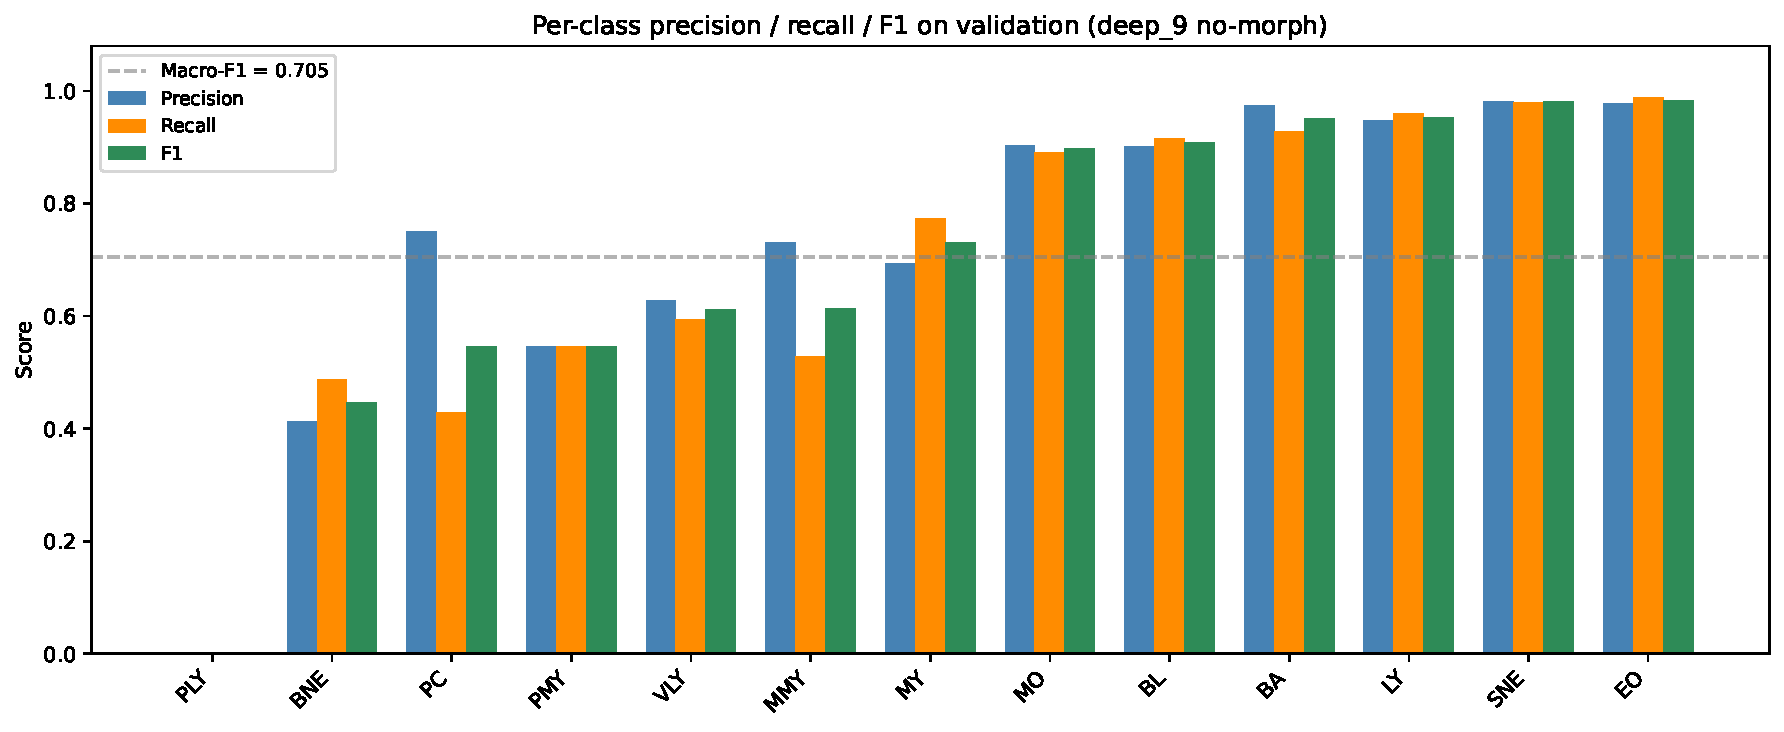
\includegraphics[width=\linewidth]{per_class_f1.pdf}
    \caption{Per-class precision, recall and F1 of the deployed model (\texttt{deep\_9 no-morph}, validation set). Dashed line = macro-F1 = 0.705.}
    \label{fig:per_class_f1}
\end{figure*}

From the deployed model's evaluation (2,891 validation images), we observe three tiers of classification difficulty:

\textbf{Well-classified} (F1 $\geq$ 0.89): EO (0.983), SNE (0.981), LY (0.953), BA (0.951), BL (0.909), MO (0.897). These have abundant data or highly distinctive morphology (BA with dark granules, EO with bilobed nucleus).

\textbf{Moderate} (F1 0.54--0.75): MY (0.731), MMY (0.613), VLY (0.611), PC (0.545), PMY (0.545). Limited training data combined with morphological overlap.

\textbf{Critical} (F1 $<$ 0.50): BNE (0.447), PLY (0.000). BNE vs.\ SNE differs only in nuclear segmentation degree. PLY has only 11 training images (1 in validation), making reliable classification impossible.

\subsection{Confusion Analysis}

\begin{figure*}[tbp]
    \centering
    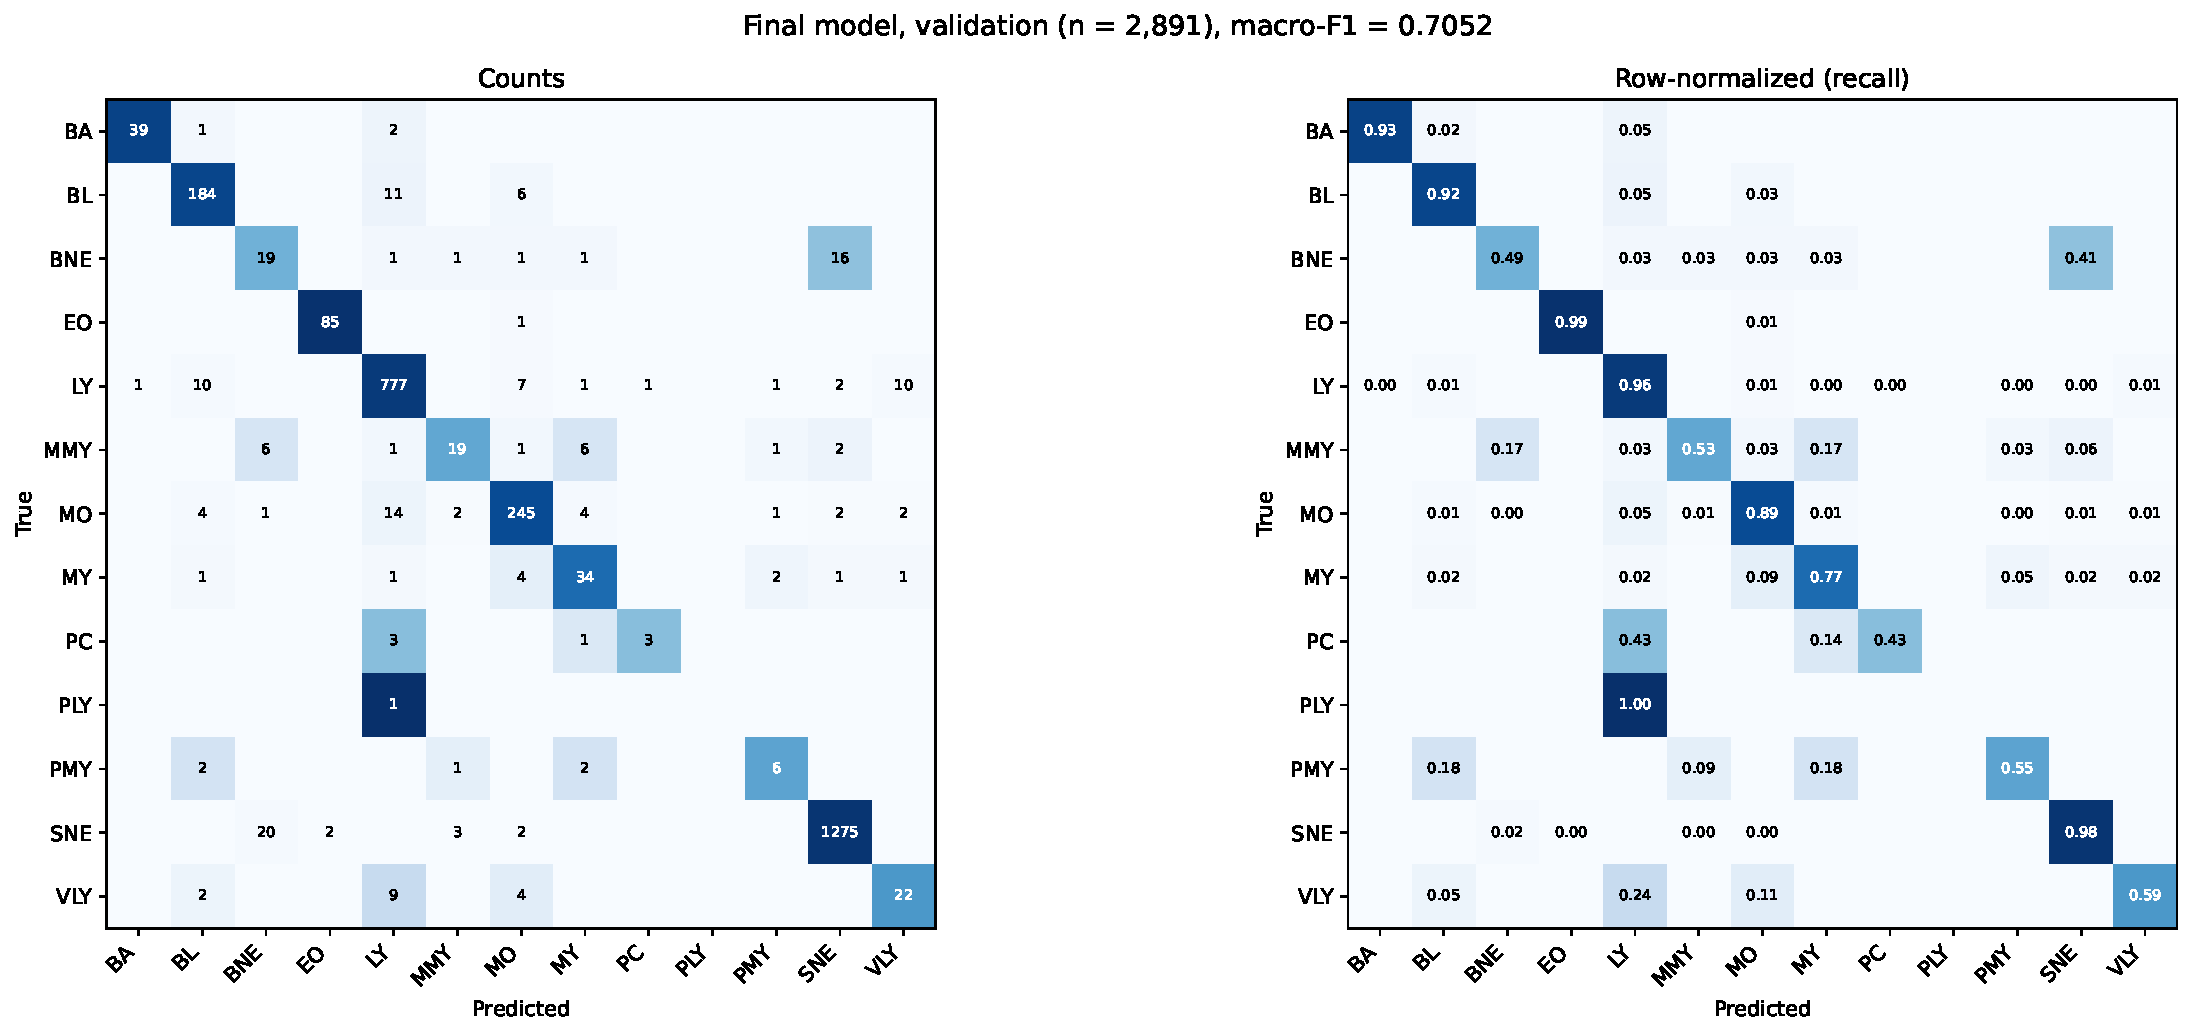
\includegraphics[width=0.9\textwidth]{confusion_matrix.pdf}
    \caption{Confusion matrix (counts and normalized recall) from the deployed model (\texttt{deep\_9 no-morph}).}
    \label{fig:confusion_matrix}
\end{figure*}

The confusion matrix reveals biologically meaningful patterns:

\begin{enumerate}
    \item \textbf{BNE $\leftrightarrow$ SNE} (SNE$\to$BNE 20, BNE$\to$SNE 16, i.e.\ 41.0\% of BNE): Band and segmented neutrophils share the same lineage, differing only in nuclear segmentation degree---a distinction that challenges even expert hematologists.
    \item \textbf{Lymphoid/mononuclear cells} (MO$\to$LY 14, BL$\to$LY 11, LY$\to$VLY 10, LY$\to$BL 10, VLY$\to$LY 9, i.e.\ 24.3\% of VLY): lymphocytes, variant lymphocytes, blasts and monocytes are all mononuclear cells with overlapping size and chromatin appearance.
    \item \textbf{Granulocyte maturation chain} (MMY$\to$MY 6, MMY$\to$BNE 6): successive maturation stages with gradually evolving nuclear shape (round $\to$ indented $\to$ bean-shaped $\to$ band).
\end{enumerate}

These confusions are consistent with genuine biological continua between neighbouring classes.

\subsection{Qualitative Error Analysis}
\label{sec:qualitative_errors}

To complement the confusion matrix, we inspected representative misclassified validation images. Figure~\ref{fig:qualitative_errors} shows the four errors made with the highest confidence; three of them confuse neighbouring stages or subtypes of the same lineage (band vs.\ segmented neutrophil, blast vs.\ lymphocyte, prolymphocyte vs.\ lymphocyte).

\begin{figure}[h]
    \centering
    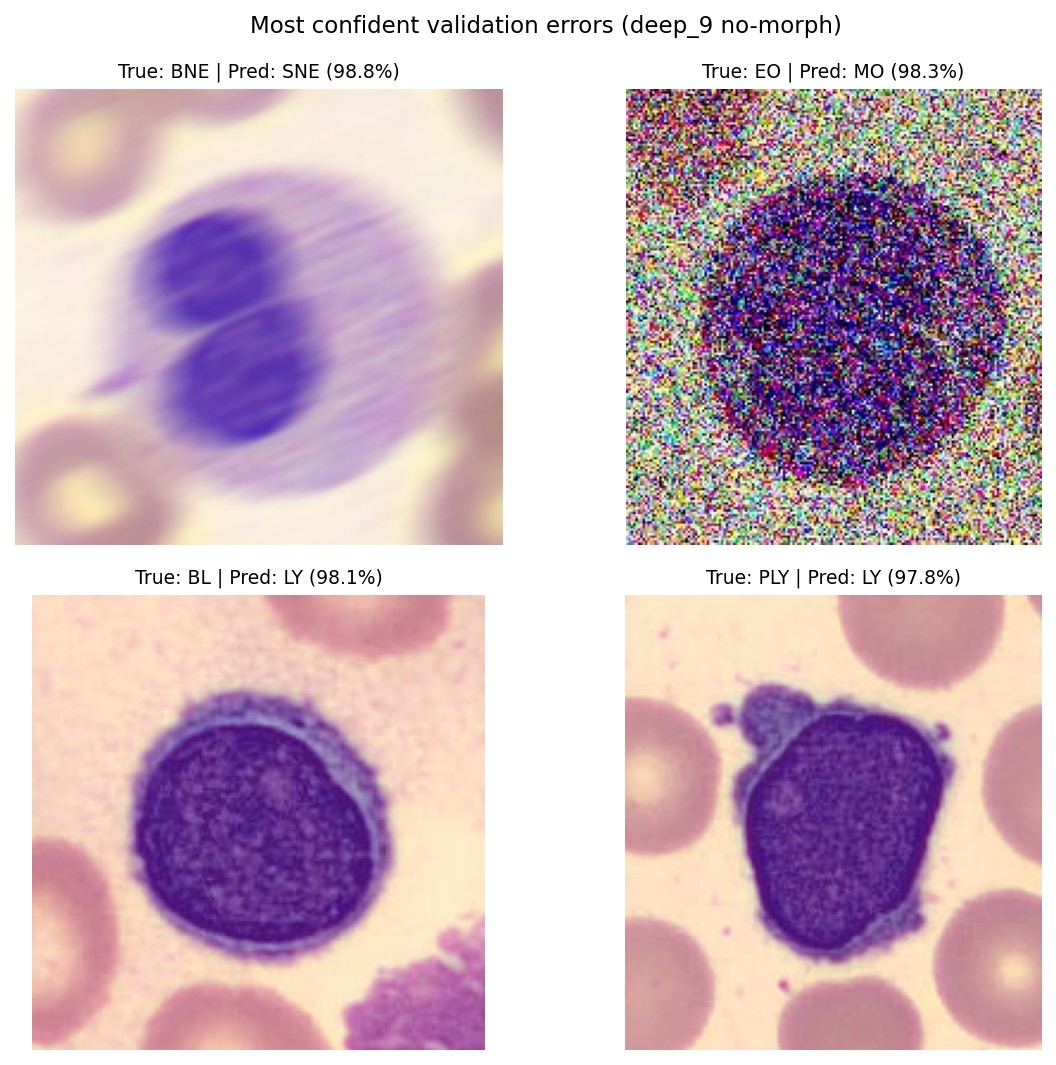
\includegraphics[width=\linewidth]{qualitative_errors.jpg}
    \caption{The four most confident validation errors of the deployed model (\texttt{deep\_9 no-morph}): BNE predicted as SNE, EO as MO, BL as LY and PLY as LY, each with a confidence above 97\%.}
    \label{fig:qualitative_errors}
\end{figure}

Three of these errors involve neighbouring classes with borderline morphology (partially segmented nucleus, intermediate chromatin condensation). The eosinophil predicted as a monocyte (top right) is heavily degraded by noise: image quality, not only class overlap, also causes errors.

\subsection{Why Deep Learning Outperforms Classical ML}

The performance gap (0.705 on a held-out split vs.\ 0.509 in cross-validation; the protocols differ, but the gap is far larger than their difference) likely comes from three factors:

\begin{enumerate}
    \item \textbf{Segmentation robustness}: The DL pipeline only needs a coarse HSV crop, which tolerates imprecise boundaries, while classical ML requires precise nucleus/cytoplasm boundaries; every segmentation failure corrupts the entire feature vector.
    \item \textbf{Feature learning}: ConvNeXt learns hierarchical features capturing subtle chromatin patterns, granule distributions, and nuclear texture at multiple scales---information that GLCM or LBP can only partially encode.
    \item \textbf{Transfer learning}: ImageNet pre-training provides general visual representations (edges, textures, shapes) that transfer well to microscopy, compensating for the limited medical training data.
\end{enumerate}

\subsection{Lessons from the Iterative Journey}

The 9-iteration journey yielded several generalizable insights:

\begin{enumerate}
    \item \textbf{The backbone mattered more than added modules}: The single largest performance jump came from switching EfficientNet-B3 (12M) to ConvNeXt-Base (88M). Size alone does not seem to be the explanation: ResNeXt101 ($\sim$87M, \texttt{deep\_8}) with CBAM, fusion and multi-task heads reached only 0.665, although it differs from \texttt{deep\_6} in several respects. None of the attention, fusion or multi-task designs we tried closed that gap.
    \item \textbf{Handcrafted features did not help ConvNeXt}: Late fusion gave a small gain with EfficientNet-B3 (\texttt{deep\_3} vs.\ \texttt{deep\_2}, $+0.008$, within noise), and the ResNet50 and ResNeXt101 models relied on their morphology branch (zero-out ablations at inference: $-0.017$ and $-0.173$), but the branch made no difference for ConvNeXt-Base (\texttt{deep\_9} with-morph vs.\ no-morph: 0.0016).
    \item \textbf{Data leakage is insidious}: The \texttt{deep\_5} $\to$ \texttt{deep\_6} episode (0.82 $\to$ 0.70) demonstrates how splitting after oversampling can create subtle leakage. Always split by original image identity.
    \item \textbf{Simplicity wins, mostly}: The deployed model (\texttt{deep\_9 no-morph}) is \texttt{deep\_6}'s backbone + MLP plus a lightweight SE gate, CLAHE preprocessing and a stronger augmentation, for a difference within noise ($+0.006$ F1, 0.7052 vs.\ 0.6994). Heavier designs (CBAM, spatial attention, multi-task, late fusion) added engineering complexity without consistent gains.
    \item \textbf{Hybrid classifiers suit small models}: CNN+SVM/RF outperformed end-to-end training for EfficientNet-B3 (\texttt{deep\_2}/\texttt{3}) but not for ConvNeXt-Base, suggesting that larger backbones produce better-separated feature spaces that don't need kernel methods.
\end{enumerate}

\subsection{Computational Cost and Clinical Feasibility}

Although ConvNeXt-Base is a large model ($\sim$88M parameters), the offline HSV cropping stage substantially reduces irrelevant background and accelerates training/inference. In our implementation, moving from online to offline cropping removed the main preprocessing bottleneck (\texttt{deep\_5} onwards); the deployed model trains at $\approx$84\,s/epoch with a frozen backbone and $\approx$140\,s/epoch during fine-tuning on a single RTX~3090.

At inference, the deployed pipeline performs a single forward pass per crop (plus optional TTA for leaderboard scoring). This makes the non-TTA mode suitable for near-real-time triage scenarios, while TTA can be reserved for high-confidence offline batch reporting.

\begin{figure*}[tbp]
    \centering
    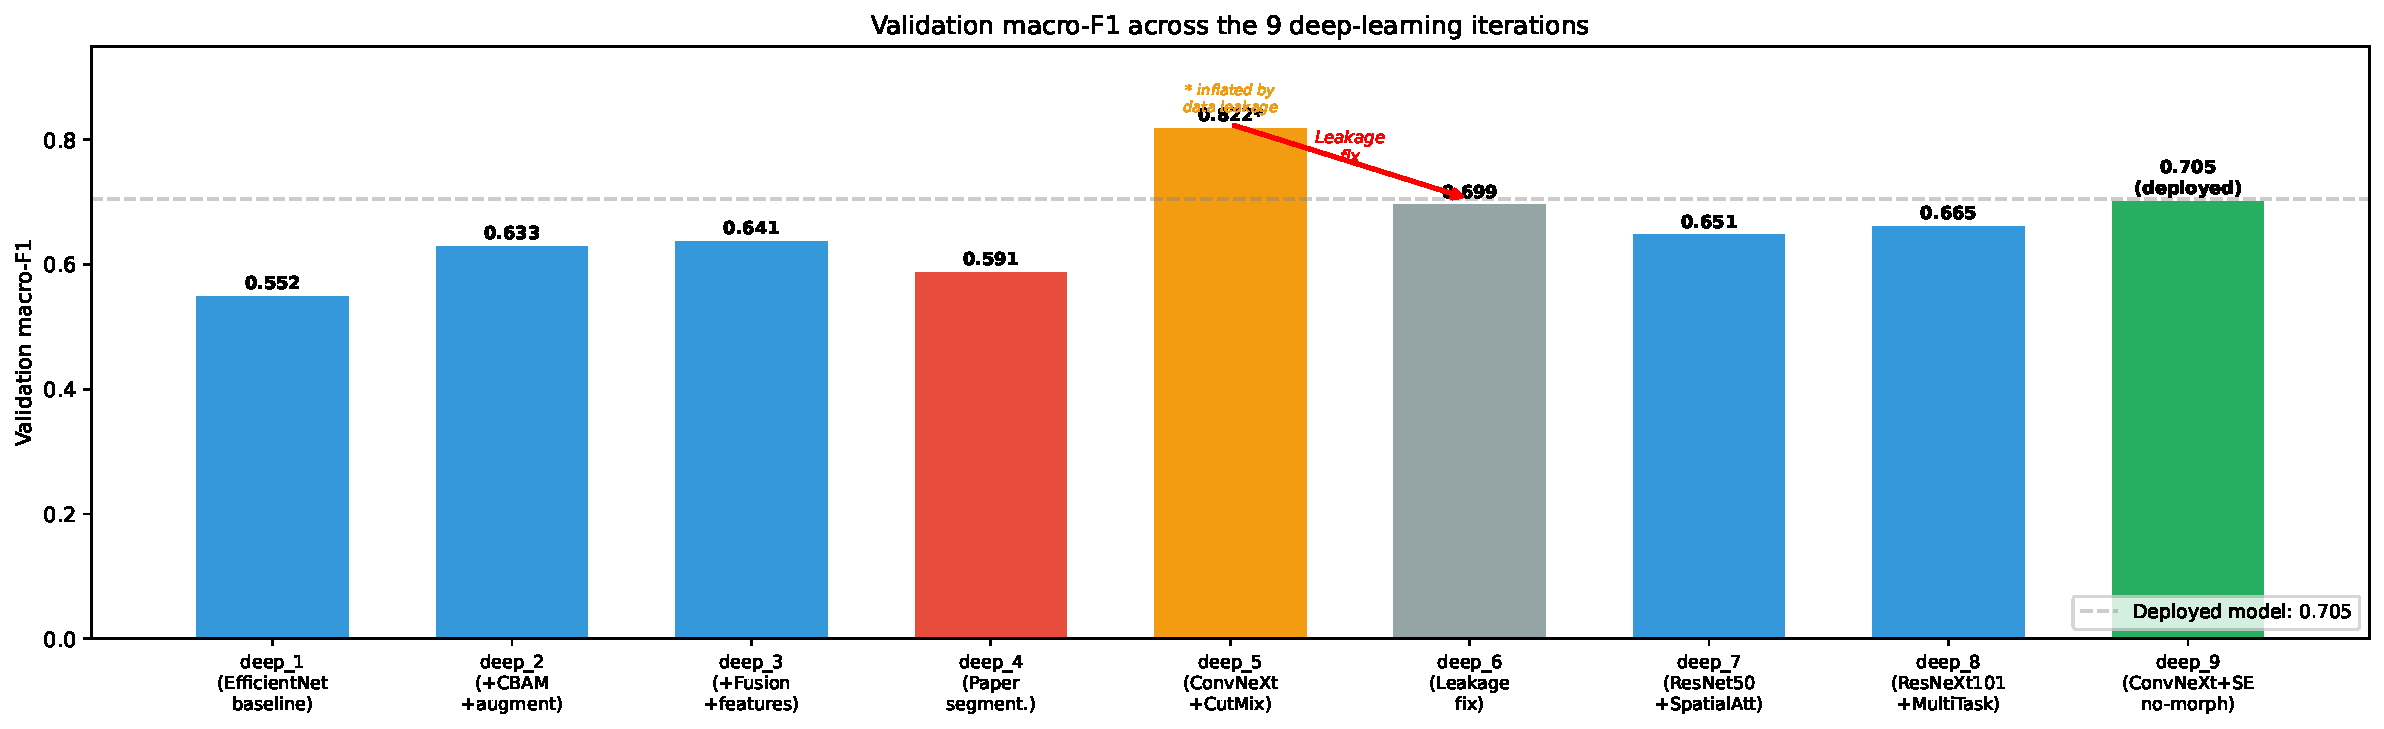
\includegraphics[width=\linewidth]{iteration_timeline.pdf}
    \caption{Validation macro-F1 across iterations. The \texttt{deep\_5}$\to$\texttt{deep\_6} drop reflects the leakage correction, not a regression. Validation sets differ between \texttt{deep\_1}--\texttt{deep\_4} and \texttt{deep\_6}--\texttt{deep\_9} (see Table~\ref{tab:iterations}).}
    \label{fig:iteration_timeline}
\end{figure*}

% ============================================================
\section{Conclusion and Future Work}
% ============================================================

We explored both classical ML and deep learning for 13-class WBC classification through an extensive iterative process spanning 9 deep learning experiments. The classical approach, while providing interpretable features, is fundamentally limited by segmentation failures and the expressiveness gap between handcrafted and learned features.

The deep learning journey revealed that the most effective design is close to the simplest one tried. After exploring CBAM attention (\texttt{deep\_2}), late fusion with handcrafted morphometry (\texttt{deep\_3}, \texttt{7}, \texttt{8}, \texttt{9}), 4-channel RGBM input (\texttt{deep\_3}), Wiener/Laplacian preprocessing (\texttt{deep\_3}), paper-based segmentation (\texttt{deep\_4}), spatial attention (\texttt{deep\_7}), multi-task auxiliary heads (\texttt{deep\_8}), and confusion-aware margin penalties (\texttt{deep\_8}), the deployed model (\texttt{deep\_9 no-morph}) is:

\begin{enumerate}
    \item \textbf{ConvNeXt-Base backbone} with ImageNet transfer learning (88.5M parameters in total).
    \item \textbf{Lightweight SE-style attention gate} on pooled features (263K params) -- with CLAHE and a stronger augmentation, the only changes from \texttt{deep\_6}, for a difference within noise.
    \item \textbf{3-layer MLP head} ($1024 \to 512 \to 256 \to 13$).
    \item \textbf{Offline HSV cropping} for robust background removal, followed by \textbf{CLAHE on the HSV V channel} at train and test time.
    \item \textbf{Focal Loss + CutMix/Mixup} for class imbalance, with rare-class protection.
    \item \textbf{2-phase training} (5-epoch frozen warmup, then full fine-tuning).
    \item \textbf{Leakage-free evaluation} with original-identity-based splits.
\end{enumerate}

This achieves macro-F1 = 0.705 on validation, outperforming classical ML (0.509) and the initial DL baseline (0.552). The iterative journey demonstrated that \textit{the choice of backbone and a sound evaluation protocol mattered more than architectural complexity} -- attention and fusion did not bring a measurable gain.

Future directions include: (1)~higher input resolution ($384\times384$), (2)~stain-specific augmentation (HSV shifts, RGBShift), which the deployed model does not use, (3)~multi-backbone ensemble (ConvNeXt + EfficientNetV2 + Swin Transformer), (4)~hierarchical classification exploiting the granulocyte maturation chain (PMY$\to$MY$\to$MMY$\to$BNE$\to$SNE), (5)~Macenko stain normalization~\cite{macenko2009} as preprocessing, and (6)~external data or synthetic generation (GANs/diffusion) for the PLY class (only 11 images).

\bibliographystyle{unsrt}
\bibliography{references}

\end{document}
